%%%%%%%%%%%%%%%%%%%%%%%%%%%%%%%%%%%%%%%%%%%%%%%%%%%%%%%%%%%%%%%%%%%%%
%%                                                                 							%%
%%		Trabajo Fin de GRADO		                       				%%
%%		TITULO 																			%%
%%		AUTOR												%%
%%                                                                 							%%
%%%%%%%%%%%%%%%%%%%%%%%%%%%%%%%%%%%%%%%%%%%%%%%%%%%%%%%%%%%%%%%%%%%%%

%%  Include con la definicion de estilos por el usuario
%%%%%%%%%%%%%%%%%%%%%%%%%%%%%%%%%%%%%%%%%%%%%%%%%%%%%%%%%%%%%%%%%%%%%

\input definl

%%  Paqueteria necesaria de fabrica
%%%%%%%%%%%%%%%%%%%%%%%%%%%%%%%%%%%%%%%%%%%%%%%%%%%%%%%%%%%%%%%%%%%%%
\usepackage{hyperref}
\usepackage{palatino}
\usepackage[dvips]{graphicx} 	  % para importar combinados latex
\usepackage{color}          		      % para importar dibujos coloreados
\usepackage{rotating}        		  % para usar \begin{sideways} que rota tabla 90 grados 
\usepackage{epsfig}          		  % para rotar figuras de Xfig  poniendo % \begin{sideways} 
\usepackage{amsmath}         	  % para usar matrix y pmatrix environment
\usepackage{stmaryrd}        		  % para usar la \bigsqcap
\usepackage{verbatim}        		  % para poner salidas de pantallas
\usepackage{listings}       	 	  % para imprimir codigo fuente
\usepackage{shortvrb}				  % 
\usepackage{url}						  % 
\usepackage{subfigure}			  % 
\usepackage[usenames,dvipsnames]{xcolor}
\usepackage{float}

  

%%%%%%%%%%%%%%%%%%%%%%%%%%%%%%%%%%%%%%%%%%%%%%%%%%%%%%%%%%%%%%%%%%%%%
%%  Configuracion de paquetes
%%%%%%%%%%%%%%%%%%%%%%%%%%%%%%%%%%%%%%%%%%%%%%%%%%%%%%%%%%%%%%%%%%%%%
\renewcommand\lstlistingname{Listado}                   %  default is Listing
%\renewcommand\lstlistlistingname{\'Indice de listados}  %  default is Listings 
%\renewcommand\thelstlisting{\thechapter .\arabic{lstlisting}} % captionstyle


\lstset{
  language=Java,
  stepnumber=1}

\usepackage{listings}
\usepackage{courier}
\lstset{
         basicstyle=\scriptsize\ttfamily, % Standardschrift
         numbers=left,               % Ort der Zeilennummern
         numberstyle=\scriptsize,          % Stil der Zeilennummern
         %stepnumber=2,               % Abstand zwischen den Zeilennummern
         numbersep=5pt,              % Abstand der Nummern zum Text
         tabsize=2,                  % Groesse von Tabs
         extendedchars=true,         %
         breaklines=true,            % Zeilen werden Umgebrochen
         keywordstyle=\bfseries\color{blue},
            frame=b,
 %        keywordstyle=[1]\textbf,    % Stil der Keywords
 %        keywordstyle=[2]\textbf,    %
 %        keywordstyle=[3]\textbf,    %
 %        keywordstyle=[4]\textbf,   \sqrt{\sqrt{}} %
         stringstyle=\color{white}\ttfamily, % Farbe der String
         showspaces=false,           % Leerzeichen anzeigen ?
         showtabs=false,             % Tabs anzeigen ?
         xleftmargin=17pt,
         framexleftmargin=17pt,
         framexrightmargin=5pt,
         framexbottommargin=4pt,
		 emph={},
		 emphstyle={\color{black}\bfseries},
         %backgroundcolor=\color{lightgray},
         showstringspaces=false      % Leerzeichen in Strings anzeigen ?        
}

%\captionsetup[lstlisting]{singlelinecheck=false, labelfont={blue}, textfont={blue}}
\usepackage{caption}
\DeclareCaptionFont{white}{\color{white}}
\DeclareCaptionFormat{listing}{\colorbox[cmyk]{1, 1, 1,0.01}{\parbox{\textwidth}{\hspace{15pt}#1#2#3}}}
\captionsetup[lstlisting]{format=listing,labelfont=white,textfont=white, singlelinecheck=false, margin=0pt, font={bf,footnotesize}}


%%  Configuraciones varias
%%%%%%%%%%%%%%%%%%%%%%%%%%%%%%%%%%%%%%%%%%%%%%%%%%%%%%%%%%%%%%%%%%%%%
\newcommand{\corregir}{\color{blue}}  	 	% pintar en color azul
\setlength{\parskip}{2ex}              			% despues del parrafo, doble linea


% Para que no aparezcan las cabeceras de las páginas que están en blanco
%%%%%%%%%%%%%%%%%%%%%%%%%%%%%%%%%%%%%%%%%%%%%%%%%%%%%%%%%%%%%%%%%%%%%
\makeatletter 
\def\cleardoublepage{\clearpage\if@twoside \ifodd\c@page\else
  \hbox{} 
  \thispagestyle{empty} 
  \newpage
  \if@twocolumn\hbox{}\newpage\fi\fi\fi} 
\makeatother

%%  Cortes de palabras especiales
%%%%%%%%%%%%%%%%%%%%%%%%%%%%%%%%%%%%%%%%%%%%%%%%%%%%%%%%%%%%%%%%%%%%%
\hyphenation{
ejem-plo Algo-ritmo
}


%\includeonly{titulo, prologo,intro,capitulo1}


\begin{document} 

%%  Titulo e Indices
%%%%%%%%%%%%%%%%%%%%%%%%%%%%%%%%%%%%%%%%%%%%%%%%%%%%%%%%%%%%%%%%%%%%%%
\pagenumbering{roman}
\thispagestyle{empty}

{


\thispagestyle{empty}
\begin{center}

\includegraphics[scale=.6]{img/logouhu}
\end{center}

\vspace*{0cm}
\Large 

\begin{center}

{\normalsize \sc Escuelta Técnica Superior de Ingeniería \\ de la Universidad de Huelva}

{\large \bf Grado en Ingeniería Informática}

\vspace*{1cm}

{\sc Trabajo Fin de Grado}


{\LARGE \bf Generación procedimental de mapas 2D. \\ Análisis e investigación del problema. }

\end{center} 




\vfill

\begin{center}
{\normalsize Autor: \\ {\bf Alejandro Seguí Díaz}}
\end{center}

\begin{center}
%{\footnotesize Tutores:}
{\small Tutores: }
\vspace*{0.2cm}
{\small \\  Gonzalo A. Aranda Corral \\ Daniel Márquez Quintanilla}
\end{center}
\begin{center}
{\footnotesize Huelva, 30 de junio de 2015.\\Curso académico 2014/15.}
\end{center}

\newpage
\thispagestyle{empty}
\vspace*{3.5cm}
\begin{center}
\small Puede encontrar una copia actualizada de este documento en \\
\small http://alesegdia.github.io/dungen-docs/latex/src/tfg\_dungen.pdf
\end{center}
\vfill


\newpage
\thispagestyle{empty}
\vfill



}


\clearpage
\pagestyle{plain}
\tableofcontents
\clearpage
\listoffigures

%%  Contenido del trabajo
%%%%%%%%%%%%%%%%%%%%%%%%%%%%%%%%%%%%%%%%%%%%%%%%%%%%%%%%%%%%%%%%%%%%%%
\pagenumbering{arabic}
\pagestyle{fancy}

%\chapter*{Prólogo}
\label{intro:prologo}
\addcontentsline{toc}{chapter}{Prólogo}


\chapter*{Introducción}
\label{intro:intro}
\addcontentsline{toc}{chapter}{Introducción.}

En la actualidad, los videojuegos han conseguido posicionarse en un mercado líder indiscutible a nivel internacional. En el ámbito del entretenimiento, la industria cinematográfica está dando paso a los videojuegos, que avanzan a pasos de gigante. Muchas grandes personalidades del cine se dirigen a los creadores de videojuegos para continuar su carrera. Un ejemplo claro de una persona adelantada para su época en este sentido, es George Lucas (\cite{lucasarts}), autor de la famosa saga Star Wars. George Lucas se introdujo en el mercado de los videojuegos en el 1986 con el título Labyrinth, dando paso posteriormente a otros títulos muy sonados y de culto como Monkey Island o Grimm Fandango.

Un videojuego, al igual que una película, puede contar una historia. Aún así, existen diferentes géneros de videojuegos, que van desde simulación de juegos de mesa, donde evidentemente no existe historia, o está intrínseca en el origen del mismo juego, hasta las denominadas aventuras gráficas, donde el enfoque está en la parte argumental. Es por ello que la industria del cine deja paso a los videojuegos de manera tan rápida.

\section*{Mapas y escenarios.}
\addcontentsline{toc}{section}{Mapas y escenarios}

Muchos géneros de videojuegos plantean su argumento en un escenario donde se da rienda suelta a la capacidad perceptiva del jugador, dando lugar en mayor o menor medida a que complete la historia con su imaginación. En este escenario, el jugador desarrollará las acciones que se le ofrezcan según el tipo de juego. Así, podrá completar la historia, permitiendo además en muchos casos que las acciones influyan en el desarrollo argumental del videojuego. Tipos de juegos que requieren mapas son, por ejemplo, juegos de acción, estrategia o rol entre otros.

El tipo de escenario que podemos encontrarnos en un juego es de lo más variopinto. A la hora de plantear la elaboración de un juego, se tiene en cuenta la elección del tipo de escenario. Muchas cuestiones sobre las que se basan estas elecciones radican sobre la complejidad de optimización del mismo:

\begin{itemize}
	\item Si el escenario es demasiado grande, no nos interesa renderizar el escenario completo, sino solamente la parte visible. Al proceso de optimizar el renderizado del mapa se le llama \emph{culling}\cite{culling}.
	\item Lo mismo pasa con las físicas. No nos interesa comprobar colisiones con elementos que es obvio que no van a colisionar. Ésto también ha de ser tenido en cuenta a la hora de elaborar el sistema de escenarios.
	\item El \emph{nivel de detalle} (Level of detail por el inglés \cite{lod}) es otro aspecto a tener en cuenta. Si una geometría está demasiado lejana del jugador, no necesitamos renderizarla exactamente como es. Este aspecto es relevante a los juegos 3D principalmente.
	\item La división o no del escenario por zonas. Esto puede evitarnos la necesidad de presencia en memoria de un mapa completo, pudiéndolo dividir en partes para ahorrar en el preciado recurso que es la memoria. Es un aspecto a tener en cuenta sobre todo cuando se elaboran juegos para videoconsolas, las cuales suelen contar con una memoria muy limitada.
\end{itemize}

Así, se exponen dos criterios principales como forma de clasificar los tipos de escenario:

\begin{itemize}
	\item Organización del escenario. Este criterio se refiere a la existencia de cortes en el desarrollo del juego para la carga de las distintas partes del mundo en el que se desarrolla el juego. Algunos tipos son:
	\begin{itemize}
		\item Escenarios totalmente continuos continuos representando un mundo totalmente abierto sin cortes. Ejemplos son \emph{GTAV} o \emph{Minecraft}.
		\item Dividido por zonas donde no existen cortes en la misma zona. Un ejemplo es \emph{Borderlands}.
		\item Dividido por zonas donde pueden existir cortes en la misma para interiores. Un ejemplo es \emph{Skyrim}.
	\end{itemize}
	\item Composición del escenario. Nos referimos a si la geometría empleada ayuda de forma implícita al manejo a nivel computacional del escenario. Algunos tipos son:
	\begin{itemize}
			\phantomsection \label{maptiles-r}
		\item Escenarios en 2D discretizados en \emph{tiles}. Básicamente, la geometría está representada por una matriz de dos dimensiones, donde cada casilla de la matriz está relacionada con una textura (o porción de la misma), siendo todas las texturas del mismo tamaño para la misma matriz. A cada casilla, la denominamos \emph{tile}. Este tipo de escenarios son muy fácilmente optimizables. Ejemplos de este tipo es, por ejemplo, \emph{Final Fantasy VI}, así como multitud de juegos de las consolas de 8 y 16 bits como la \emph{NES} o \emph{SNES}.
		\item Una extensión a 3D de los escenarios de tiles son los escenarios compuestos por \emph{voxels} \cite{voxel}. Estos han sido recientemente popularizados por el famoso título \emph{Minecraft}, donde el escenario está gestionado por un \emph{motor de voxels} que ayuda a optimizar tanto con culling como con físicas.
		\item Escenarios con geometría deliberada. Es decir, la geometría (ya sea 2D o 3D), no presenta ninguna propensión a ser optimizada. Este tipo de escenarios, suelen optimizarse con el uso de \emph{quadtrees} \cite{quadtree} (para 2D) u \emph{octrees} \cite{octree} (para 3D)
		\item Escenarios hechos con los denominados \emph{brushes} \cite{brush}. Esta técnica se utiliza para 3D, y consiste en el uso de geometrías convexas para componer un escenario. Ejemplos famosos de este tipo de escenarios es \emph{Quake} \cite{quake}.
	\end{itemize}
\end{itemize}

Una vez expuestos los criterios para clasificar los tipos de mapas, remarcar que hay casos en los que los desarrolladores convienen formas nuevas de organizar el mapa debido a necesidades particulares, por lo que los ejemplos expuestos en cada criterio no completan de ninguna manera las múltiples categorías para cada uno.

Para el desarrollo de este proyecto y atendiendo a las especificaciones presentadas en el capítulo~\ref{cap:capitulo2}, abarcaremos \emph{mapas de tiles} para el género de juego \emph{roguelike} \cite{rlike}. Este género se caracteriza precisamente por mapas generados de forma procedimental. Cada nivel es entendido como una planta, donde el jugador tiene que llegar desde donde aparece hasta un tile considerado como final para poder continuar hasta la siguiente planta. Así, el jugador va avanzando niveles hasta que llega al último y completa el juego al finalizar el mismo.



\section*{Motivación y Objetivos.}
\addcontentsline{toc}{section}{Motivación y Objetivos}

Como se ha mencionado previamente, la industria de los videojuegos avanza a pasos de gigante. Es por ello que las compañías invierten cada vez más en videojuegos, siendo a veces el coste en marketing superior al de desarrollo \cite{costgames}. Existe un amplio espectro de puestos encontrados en este campo \cite{gdroles1} \cite{gdroles2}, entre los cuales existen

\begin{itemize}
	\item \emph{Game programmer}. Personal dedicado a la programación de las mecánicas del juego, eventos y otros relacionados con el propio juego
	\item \emph{Core programmer}. Personal dedicado a la elaboración del motor que será la base sobre la que funcionará el juego. Normalmente se subdivide en subroles como \emph{graphics programmer} o \emph{physics programmer}. En muchos casos, se parte de un motor ya elaborado sobre el que se realizan las modificaciones necesarias para el juego en cuestión.
	\item \emph{Game designer}. Dedicados a la elaboración de las mecánicas del juego, así como el plot del mismo.
	\item \emph{Level designer}. Personal dedicado exclusivamente a la elaboración de escenarios empleando programas externos o el mismo motor que se esté utilizando, si éste posee dichas capacidades.
	\item \emph{AI programmer}. Dedicado a la programación de los distintos sistemas de inteligencia artificial existentes en el juego.
	\item \emph{Muchos más...}
\end{itemize}

En este listado, solo hemos tenido en cuenta algunos de los puestos del aspecto de desarrollo, pero quedaría añadir muchos más como diseñadores gráficos y apartado de marketing.

Destacar que el \emph{level designer}, pese a que no se encarga de la construcción de las herramientas para crear el escenario, debe conocer las bases del tipo de escenario que se empleará en el juego, de forma que adapte sus técnicas de diseño al tipo de escenario y así poder optimizarlos en la medida de lo posible.

Recientemente, y debido a las cada vez más crecientes facilidades para crear un videojuego, han surgido los llamados \emph{equipos indies} \cite{gdindie}, caracterizados principalmente por tener un bajo presupuesto y personal. Normalmente suelen empezar con un presupuesto nulo, pero en algunos casos llegan a triunfar de manera inesperada incluso por los mismos desarrolladores. Ejemplos son \emph{Hotline Miami}, \emph{Minecraft} o \emph{Risk of Rain}.

Los equipos con un presupuesto considerable (coloquialmente denominados AAA), no tienen problemas a la hora de contratar \emph{diseñadores de niveles}, ya que disponen de una gran cantidad de dinero para depositar en los distintos roles necesarios para un juego. Aún así, en combinación con un generador de mapas, un \emph{diseñador de niveles} puede desarrollar ideas que den un resultado muy bueno. Ejemplos de esto son \emph{Diablo} o \emph{Torchlight}, donde los mapas son generados automáticamente partiendo de patrones elaborados a mano por \emph{diseñadores de niveles}.

Así, el la motivación de este proyecto reside en dos ideas principales.

\begin{itemize}
	\item Ahorro de coste y tiempo para equipos indies, que no pueden permitirse el lujo de gastar en personal exclusivo para el diseño de niveles.
	\item Adición de variedad a los escenarios de juegos, permitiendo incluso a un equipo de desarrolladores AAA
\end{itemize}


\section*{Solución Propuesta.}
\addcontentsline{toc}{section}{Solución Propuesta}

La solución que se propone es un sistema capaz de generar escenarios de manera automática con una mínima interacción (o incluso nula si se desea) de los diseñadores. Esto además, conlleva dinamismo en los escenarios que se podrán jugar, de forma que de partida a partida, la distribución del escenario será completamente distinta.

La elaboración de un generador de escenarios, une las competencias de dos roles en el desarrollo de videojuegos:

\begin{itemize}
	\item \emph{Diseñador de niveles.} Se necesitan conocimientos sobre la composición de los escenarios del juego, además de las propiedades concretas en cuanto a los criterios mencionados anteriormente.
	\item \emph{Programador de IA}. La creación del sistema que genere los escenarios es un trabajo que compete a este rol, ya que estamos tratando de resolver un problema donde las posibilidades de resolución son casi infinitas.
\end{itemize}

Finalmente, se elaborará el sistema reduciendo el problema a una búsqueda, donde el \emph{espacio de estados} son todas las posibles combinaciones de habitaciones conectadas.

\section*{Estructura de la memoria.}
\addcontentsline{toc}{section}{Estructura de la memoria}

Esta memoria se estructura en varios capítulos, con la siguiente distribución de los temas trabajados:

\begin{itemize}
	\item Capítulo~\ref{cap:capitulo1}. Mostraremos el origen y estado actual del campo de generación procedimental de contenido.
	\item Capítulo~\ref{cap:capitulo2}. Definiremos el problema junto con sus especificaciones y requisitos. Se comentará el tipo de juego al que se ha enfocado y el tipo de mapa utilizado.
	\item Capítulo~\ref{cap:capitulo3}. Analizaremos en profundidad la representación del modelo de datos elegida para el desarrollo del generador propuesto.
	\item Capítulo~\ref{cap:capitulo4}. Desarrollo de la estrategia empleada para el generador. Como se podrá comprobar, se ha utilizado una estrategia flexible sobre la que posteriormente, construiremos el método de búsqueda.
	\item Capítulo~\ref{cap:capitulo5}. Detalle de la implementación basada en búsqueda. Analizaremos cada uno de los elementos empleados tanto para la generación del mapa, como para la adición de diversidad.
	\item Capítulo~\ref{cap:capitulo6}. Una vez explicada la estrategia, en este capítulo se desarrollará una correspondencia entre el método de búsqueda y la estrategia implementada basada en el mismo.
	\item Capítulo~\ref{cap:capitulo7}. Comparación y análisis del impacto de diversos componentes que se han empleado para promover tanto la diversidad como la eficiencia.
	\item Capítulo~\ref{cap:capitulo8}. Posible trabajo futuro pertinente a la elaboración de una aplicación comercial con el método expuesto en este proyecto
	\item Bibliografía.
\end{itemize}

\chapter{Estado del arte.}\label{cap:capitulo1}

En este capítulo, analizaremos el ámbito de la generación procedimental de contenido para videojuegos. Veremos las distintas subdisciplinas presentes, así como los problemas que resuelven. Se hará hincapié en la generación de escenarios, ya que es el campo que compete al proyecto.

\section{Generación de contenido procedimental.}

Más conocida por su nombre en inglés (Procedural Content Generation), se refiere a la disciplina de generar contenido partiendo de algoritmos, en lugar de hacerlo manualmente.

Tuvo sus inicios en la subcultura informática llamada \emph{Demoscene} \cite{dmscn}. Este movimiento tuvo sus inicios a finales de los años 70 y principios de los 80, y continúa a día de hoy. Consiste en crear contenido visual y sonoro de forma programada, ya sea en parte o en su totalidad, y tenía como uno de sus objetivos escudriñar al máximo las limitadas capacidades de los ordenadores de la época.

Los \emph{sceners} de este campo, conseguían generar contenidos que eran impensables para la época, como por ejemplo escenas en 3D cuando a OpenGL aún le quedaban un par de décadas para aparecer. Por su habilidad, la mayoria de los demosceners terminaban trabajando para empresas de videojuegos de la época, cuando aún no había tantas facilidades a la hora de crearlos.

Existen diversas subdisciplinas en las que se aplica el concepto de generación procedimental de contenido:

\begin{itemize}
	\item \emph{Escenarios}.
	\item Texturas \cite{texmodproc}. Un ejemplo de ello es la generación de texturas que imitan el mármol o la madera. En algunos casos se emplean autómatas celulares.
	\item Geometría. Generación de follaje, o árboles empleando L-Systems. \cite{texmodproc}
	\item Mecánicas. El juego Left4Dead y su secuela, emplean un sistema procedimental para gestionar los momentos de tensión y la dificultad de las situaciones según las acciones que han ido tomando los jugadores.
\end{itemize}

Otra clasificación de los métodos procedimentales es según el momento de ejecución del procedimiento. Si el procedimiento es ejecutado antes del lanzamiento del juego, o después con la particularidad de que se realiza en servidores ajenos al jugador, lo denominaremos \emph{offline}. Sin embargo, si el procesamiento se realiza en el sistema en que se está ejecutando el juego, lo llamaremos \emph{online}.

\section{Generación de mapas.}

La generación de escenarios se considera un concepto muy amplio, ya que según el contexto del juego, puede variar bastante. Por ejemplo, en un juego ambientado en el espacio exterior, el escenario puede entenderse como una galaxia completa, como es el caso de \emph{Elite: Dangerous}.

Otro tipo de modelo a usar en la generación de escenarios es el ruido Perlin. Éste puede ser muy útil en conjunto con el concepto de mapas de alturas para generar terrenos al aire libre montañosos \cite{libnoise}. También se ha empleado el \emph{algoritmo de Voronoi} para la generación de terrenos \cite{amitvoronoi}.

Algún ejemplo más histórico de generación de escenarios pueden ser los múltiples algoritmos de generación de laberintos que se conocen \cite{labygen}.

Debido a que los métodos anteriores son demasiado genéricos, una opción muy popular es idear y construir un generador específico para el juego en cuestión que se esté desarrollando. Un ejemplo de ello es \emph{TinyKeep}, cuyo autor describe a grandes rasgos en \cite{tinykeep} las fases y el desarrollo del algoritmo que ha creado. Esta opción es la que se desarrollará en este proyecto, procurando mantener un nivel de genericidad y capacidad de personalización del sistema.



   % 
\chapter{Especificaciones.}\label{cap:capitulo2}

Definiremos las especificaciones y directrices tanto del tipo de juego como del sistema de generación. Dichas directrices que delimitarán el sistema a crear, han sido establecidas por la empresa indie de videojuegos \emph{TheGameKitchen}, y el sistema será empleado en un futuro título de la misma.

\section{Género de juego.}

En esta sección abarcaremos el tipo de juego y las directrices establecidas en cuanto al género de juego y otras especificaciones relacionadas con el mundo en el que se desarrollará el mismo.

\subsection{Roguelike}

El género de juego en el que nos basaremos será \emph{roguelike} \cite{rlike}, cuyas características principales son:

\begin{itemize}
	\item \emph{Generación de mazmorras}. Cada vez que el jugador inicia una partida, la experiencia será ligeramente distinta.
	\item \emph{Importancia considerable a la exploración}. El hecho de que las mazmorras no sean siempre iguales, incita al jugador a tener que invertir tiempo en explorar para poder encontrar la salida.
	\item \emph{Desarrollo del juego por plantas}. El objetivo del jugador suele ser llegar a una habitación considerada como final, donde puede elegir entre tomar las escaleras para pasar a una siguiente planta, o investigar un poco más en la presente.
	\item \emph{Dificultad progresiva}. Cada planta, tendrá una dificultad ligeramente mayor a la de la anterior hasta llegar a la última.
	\item \emph{Muerte permanente}. Una vez que el jugador muere, no hay manera de cargar la partida. La unica opción es comenzar de nuevo.
\end{itemize}

Históricamente, el género \emph{roguelike} se identificaba además por otro tipo de características, como la mecánica por turnos o el énfasis en jugabilidad y desinterés en los gráficos, pero con el tiempo, el género se ha ido abriendo paso a una definición más genérica. Debido a ésto, hoy en día existen desde \emph{shooters} considerados \emph{roguelike}, como por ejemplo \emph{Tower of Guns} o \emph{Paranautical Activity}, hasta \emph{plataformas}, como \emph{Risk of Rain} o \emph{Spelunky}.

\subsection{Especificaciones del mundo}

Así, las únicas especificaciones que se han dado en cuanto a las reglas de juego son las siguientes:

\begin{itemize}
	\item Entorno en dos dimensiones
	\item El jugador comenzará en una habitación y tendrá como objetivo llegar a una habitación final
	\item Se empleará una vista cenital (figura~\ref{fig:tileclip}).
\end{itemize}

\begin{figure}[t]
\centering
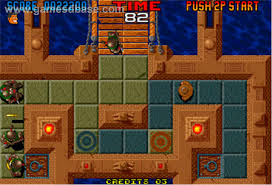
\includegraphics[scale=1]{img/cenital}
\caption{Vista cenital en el juego Action Hollywood por TCH, 1995
\label{fig:cenital}}
\end{figure}

Estas especificaciones son bastante genéricas, por lo que el sistema elaborado podrá servirnos para otro tipo de juegos. Más adelante veremos que se ha procurado dar un enfoque de alta flexibilidad en este aspecto al sistema.

\section{Requisitos del escenario.}

La representación de los escenarios elegida será un mapa de tiles. Como se comentó anteriormente, los mapas de tiles están representados por una matriz, donde cada casilla corresponde a un gráfico de un tamaño normalizado para todos los tiles (un gráfico para las paredes, otro para el suelo, etc). Suelen componerse por capas para añadir decorado, pero para nuestra finalidad, hemos obviado esta característica, ya que se hará hincapié principalmente en la distribución de las habitaciones. No obstante, sería muy sencillo añadir capas como mejora futura.

La optimización en cuanto a clipping (evitar renderizar zonas no visibles) en un mapa de tiles está muy investigada. Debido a que el propio mapa es una rejilla, se puede recorrer y renderizar exclusivamente la zona que va a verse. En la figura~\ref{fig:tileclip} se representa en rojo el viewport del jugador. Los tiles amarillos están en el borde del viewport, y los verdes están completamente dentro. Así, solo hace falta recorrer y dibujar los tiles verdes y amarillos, ahorrándonos el dibujado de los azules.

\begin{figure}[t]
\centering
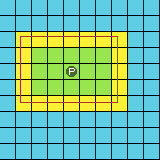
\includegraphics[scale=1]{img/tileclip}
\caption{Clipping en un mapa de tiles
\label{fig:tileclip}}
\end{figure}

Otra característica importante de los mapas de tiles es la sencillez y flexibilidad que da a la hora de componer escenarios; podemos reutilizar tiles y añadir variaciones de los mismos para, en el mapa final, dar sensación de variedad sin tener que elaborar muchos gráficos.

Por todo ello, es un tipo de escenario muy popular desde las antiguas consolas como \emph{NES} o \emph{SNES} hasta hoy.

El escenario estará compuesto por habitaciones, cada una representada como una matriz. Será nuestra tarea plantear un sistema que elabore distribuciones de las habitaciones según los requisitos que se expondrán a continuación.

\section{Directrices para la generación.}

En esta sección explicaremos las directrices impuestas para la generación de los escenarios.


\subsection{Lista inicial de habitaciones}

El sistema que construiremos deberá cumplir una serie de características que analizaremos en detalle en esta sección. Como se ha mencionado previamente, se ha tomado la libertad de añadir características que no estaban en los requisitos previos de \emph{TheGameKitchen}.

El sistema debe generar un mapa de tiles partiendo de una \emph{lista inicial de habitaciones} previamente construida. Para construir las habitaciones, se ha elaborado un editor via web usando el canvas que proporciona HTML y JavaScript (se puede ver en la figura~\ref{fig:roomed}). Así, el objetivo será colocar las habitaciones presentes en esta lista inicial.

\begin{figure}[t]
\centering
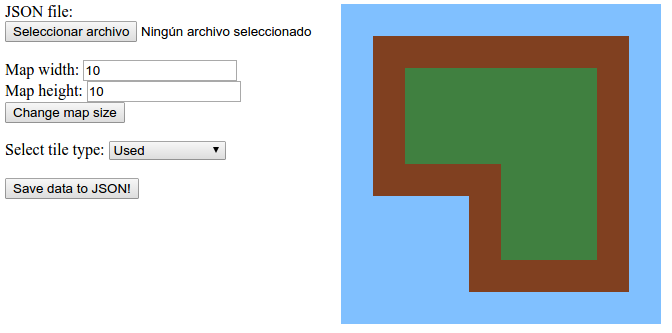
\includegraphics[scale=0.5]{img/roomed}
\caption{Editor de habitaciones
\label{fig:roomed}}
\end{figure}

Las habitaciones \emph{pueden repetirse}, es decir, si hemos creado dos modelos de habitación \emph{A} y \emph{B}, podemos tener 3 instancias del modelo \emph{A} y 2 instancias del modelo \emph{B} en la lista inicial. Hablaremos de este detalle en el próximo capítulo, que nos servirá para conseguir una mejora de optimización tanto de memoria como en procesamiento.

\subsection{Requisitos de distribución}

A continuación, explicaremos los requisitos que ha de cumplir la distribución las habitaciones.

Se ha de \emph{maximizar el camino} desde la habitación inicial hasta la habitación final. De esta forma conseguimos en parte promover que el jugador tenga que investigar.

Obviamente, se ha de conseguir una variabilidad en los niveles añadiendo un componente aleatorio, de forma que la experiencia de cada jugador (o incluso del mismo en partidas distintas) no sea idéntica.

Es indiferente que par de habitaciones son la inicial y la final, podemos elegir cualquier par.

Partiremos de un mapa de tiles vacío, cuyo tamaño supondremos suficiente como para albergar todas las habitaciones para cualquier distribución de las mismas. Para ello, es posible crear un mapa con tamaño autoajustable según sea necesario, pero se ha optado por elegir un tamaño lo suficientemente grande para hacer las pruebas.

El tamaño del escenario no sobrepasará un área de 64x64 tiles. Este tamaño no es una restricción fuerte, sino una guía para saber a qué tamaños nos enfrentaremos. Debido a esto, el área final del escenario puede ser algo menor o mayor a este tamaño de 64x64 tiles.

Se ha de fomentar la existencia de caminos alternativos, no necesariamente caminos alternativos a la solución, sino más bien callejones sin salida, de forma que incite aún más a la exploración.

\subsection{Requisitos técnicos}

La generación será \emph{online}, implicando que el sistema ha de actuar en un tiempo considerable para evitar largas esperas. Para esto, se ha construido un sistema de caché del que hablaremos más adelante.

Debe funcionar en sistemas móviles. Esto implica un especial cuidado en la optimización y en las librerías utilizadas. Para abarcar este punto correctamente, se ha utilizado Java como lenguaje de programación, ya que es el más popular para sistemas móviles. Además, el sistema de caché que se mencionó antes, nos servirá también en este aspecto.




   % 
\chapter{Representación.}\label{cap:capitulo3}




\section{Topología.}



\section{Habitaciones.}


\subsection{Puertas potenciales.}

\subsection{Prefabs.}

\subsection{Instancias.}

\subsection{Mapa.}

   % 
\chapter{Estrategia constructiva.}\label{cap:capitulo4}

Hasta ahora hemos visto la representación de las distintas entidades que entran en juego. En este capítulo introduciremos parte de la lógica que seguirá el sistema. Destacar que, aunque el enfoque final ha sido reducir el problema a una modificación de búsqueda, el sistema está pensado de forma que sea flexible a la hora de utilizar otro tipo de estrategias.


\section{Algoritmo de generación}
A la metodología que hemos utilizado la hemos denominado \emph{estrategia constructiva}, cuyo origen radica en la forma de generar el mapa. Como se puede ver en el listado \ref{lst:mlisting}, el sistema construirá el mapa por pasos. de forma que en cada paso se hará una elección de una habitación y se colocará en el mapa. Así, el sistema dará por concluida la generación cuando no queden habitaciones en la lista inicial.

\begin{lstlisting}[caption={Algoritmo constructivo para generar mapas},label={lst:mlisting},language=Java,escapechar=|]
Mapa GenerarMapa( List<Habitacion> habitaciones, InterfazSeleccion mapSolver ) {
	Mapa mapa = MapaVacio();
	while( !habitaciones.isEmpty() ) {
		List<Movimiento> movimientos = GenerarMovimientos( mapa, habitaciones ); |\label{line:movgen}|
		Movimiento elegido = mapSolver.ElegirMovimiento( ); |\label{line:ifaceselect}|
		mapa.InsertarHabitacion( elegido.habitacion, elegido.posicion ); |\label{line:addroom}|
		habitaciones.remove( elegido.habitacion ); |\label{line:rmroom}|
		GuardarMovimiento( elegido ); |\label{line:savemov}|
	}
	EstablecerRecorridoPrincipal( mapa ); |\label{line:inifin}|
	return mapa;
}
\end{lstlisting}

En el listado \ref{lst:mlisting} se introducen dos conceptos nuevos: \emph{movimientos} e \emph{interfaz de selección de movimiento}, y ambos son clave para el entendimiento del funcionamiento del sistema.

A grandes rasgos, se elige un par $(habitacion, posicion)$ y se inserta en el mapa (línea~\ref{line:addroom}). Posteriormente, se elimina la habitación de la lista de habitaciones, ya que se acaba de colocar (línea~\ref{line:rmroom}). Por último, guardamos el movimiento (línea~\ref{line:savemov}). Más adelante veremos la utilidad de ésto.

Antes de devolver el mapa, establecemos el recorrido principal (línea~\ref{line:inifin}), es decir, elegimos la habitacion inicial y final. Para ello, se ha empleado el algoritmo de \emph{Floyd-Warshall}, ayudándonos de la \emph{matriz superior de conexiones entre habitaciones} comentada en el capítuloX (INSERTARENLACE). El objetivo algoritmo \emph{Floyd-Warshall} (APENDICEINSERTARENLACE) es, dado un grafo, establecer los caminos mínimos entre todos los pares de nodos posibles. Así, para establecer el recorrido principal, elegiremos el par de nodos cuya distancia mínima sea mayor.

\section{Movimientos}

Un movimiento $M_i(R_i,P_i)$ está constituido por:

\begin{itemize}
	\item$R_i$: \emph{instancia de habitación} a colocar en el mapa
	\item$P_i$: \emph{posición} del mapa donde colocaremos dicha habitación
\end{itemize}

Así, en cada paso de colocación de una habitación, se generarán todos los movimientos posibles a realizar (listado~\ref{lst:mlisting}, línea~\ref{line:movgen}). La lista de movimientos posibles dependerá del estado del sistema, como veremos a continuación.

\subsection{Cómputo de posibles movimientos.}

Consideraremos que el \emph{estado del sistema} depende de, y se ve afectado por:

\begin{itemize}
	\item Instancias de habitación restantes en la lista inicial
	\item Modelo de instancias de habitaciones colocadas en el mapa
	\item Posición de las instancias de habitaciones colocadas
\end{itemize}

Como se observa en la figura~\ref{fig:posmovs}, dado un estado del sistema $S(map,RR)$, la lista de posibles movimientos se computará a partir de las \emph{posibles conexiones} entre las \emph{puertas potenciales de las habitaciones colocadas en el mapa} y las \emph{puertas potenciales de las habitaciones restantes}. El concepto de \emph{puerta potencial} se discutió en el CAPITLOX (insertar enlace).

\begin{figure}[h]
\centering
{
	$$S(map, RR), RR = habitacionesRestantes$$
	$$movimientos = \bigcup_{r \in RR}posiblesConexiones(map, r)$$
}
\caption{Cómputo de lista de movimientos dado un estado del sistema
\label{fig:posmovs}
}
\end{figure}

El cómputo de las posibles conexiones entre el mapa y una de las habitaciones restantes, se define en la figura~\ref{fig:poscons}. Destacar que el desplazamiento para testear la posible conexión entre una habitación de las restantes y una del mapa, solamente se puede realizar sobre la habitación restante, ya que las del mapa ya han sido colocadas y están fijas.

\begin{figure}[h]
	$$posiblesConexiones(map, r) = $$
	$$\bigcup_{p \in rooms(map)}  \left\{ cx(map,r,p,u) : \neg col(map, r, u), u \in map \right\}$$
	$$u = \begin{cases}
		u = v + (1,0) \\
		u = v - (1,0) \\
		u = v + (0,1) \\
		u = v - (0,1) \\
	\end{cases}$$
	$$col(map, room, t) : \text{colisión al colocar $room$ en $map$ en el tile $t$}$$
	$$cx(map,r,p,u) : \text{acción de conectar $r$ con $p$ colocando $r$ en tile $u$ de $map$}$$
\caption{Cómputo de las posibles conexiones entre una habitación de las restantes y el mapa
\label{fig:poscons}
}
\end{figure}

El cómputo de todos los posibles movimientos queda como la unión de los conjuntos que dan como resultado calcular las posibles conexiones entre todas las habitaciones restantes y las presentes en el mapa.

Así, el cómputo de todas las posibles conexiones entre una habitación en la lista de habitaciones restantes y una habitación del mapa consiste en calcular el conjunto de todas las posibles colocaciones de la habitación de la lista de restantes contigua a la habitación del mapa.


\section{Interfaz de selección de movimiento}

Como se ha comentado anteriormente, la \emph{interfaz de selección de movimiento} es otro elemento importante del sistema, y en ella radica parte de la flexibilidad del sistema. En el listado \ref{lst:igen} se muestra el esqueleto de dicha interfaz, cuyo único método de interés es el relacionado con la elección del movimiento.

\begin{lstlisting}[caption={Interfaz de generación},label={lst:igen},language=Java,escapechar=|]
interface InterfazSeleccion {
	Movimiento ElegirMovimiento( List<Movimiento> movimientos );
}
\end{lstlisting}

Una vez generados todos los movimientos posibles, se delega la decisión de elegir un movimiento a la \emph{interfaz de generación}. En esta interfaz radica uno de los puntos de flexibilidad del sistema. Mediante componentes que implementen esta interfaz, podemos idear otras formas de elegir un movimiento a partir de la lista de movimientos posibles.

En este proyecto se han creado dos interfaces de selección de movimiento:

\begin{itemize}
	\item \emph{Interfaz aleatoria}. Elige un movimiento de forma aleatoria de entre todos los posibles.
	\item \emph{Interfaz basada en búsqueda}. Asigna una puntuación a cada movimiento y elige la mejor.
\end{itemize}

La interfaz aleatoria es simple y no tiene interés computacional. En el listado \ref{lst:irandom} se muestra la implementación de dicha interfaz por completitud, pero se ha realizado solo para testeo.

\begin{lstlisting}[caption={Implementación aleatoria de la interfaz de selección de movimiento},label={lst:irandom},language=Java,escapechar=|]
Movimiento ElegirMovimiento( List<Movimiento> movimientos ) {
	int indiceMovimiento = random( 0, movimientos.size() - 1);
	Movimiento elegido = movimientos.get( indiceMovimiento );
	return elegido;
}
\end{lstlisting}

   % 
\chapter{Interfaz basada en búsqueda.}\label{cap:capitulo5}

En este capítulo se abarcará en cierta profundidad la \emph{interfaz de selección basada en búsqueda}. Se han omitido algunos detalles como la forma de crear y manejar las puertas, ya que se considera trivial y fuera del objetivo de la práctica. Además, algunos concepto como el concepto de \emph{movimiento} no se traduce literalmente en el código, pero la idea esencial se conserva.

En el capítulo siguiente veremos la relación de este acercamiento con el método de búsqueda.

\section{Estrategia basada en búsqueda}

Como se observa en el listado~\ref{lst:igensearch}, la forma de seleccionar el movimiento incluye el cálculo de una puntuación numérica que llamaremos \emph{fitness}. Para obtener el \emph{fitness}, aplicaremos una función que denominaremos como \emph{función guía}, y devolverá un valor numérico indicando la calidad del movimiento.

\begin{lstlisting}[caption={Interfaz de selección de movimiento basada en búsqueda},label={lst:igensearch},language=Java,escapechar=|]
class BestSearchMovementSelector implements IMovementSelector {
	Movimiento ElegirMovimiento( List<Movimiento> movimientos ) {
		List<Float> fitnesses;
		for( Movimiento m : movimientos ) {
			fitnesses[m.index] = FuncionGuia( m );
		}
		Movimiento elegido = ObtenerMejor( movimientos, fitnesses );
		return elegido;
	}
}
\end{lstlisting}

Aplicando la \emph{función guía} a todos los movimientos, se computará el \emph{fitness} para cada uno. Por último, elegiremos el movimiento cuyo \emph{fitness} sea mejor. Convendremos que la calidad del \emph{fitness} será directamente proporcional al mismo, es decir, cuanto mayor \emph{fitness}, mejor movimiento.

\section{Interfaz de cómputo de fitness}

Para el cómputo del fitness, se ha empleado una interfaz que definimos en el listado~\ref{lst:ifit}, añadiendo flexibilidad a este componente. De esta forma, podemos también idear formas nuevas de computar el fitness y llevarlas a la práctica fácilmente.

\begin{lstlisting}[caption={Interfaz de cómputo de fitness},label={lst:ifit},language=Java]
interface IFitnessSolver {
	float FuncionGuia( Movimiento m );
}
\end{lstlisting}

En el listado~\ref{lst:igsf} se ha sustituido la llamada a la función guía por la interfaz de cálculo de fitness. De esta forma, añadimos un componente de flexibilidad en esta parte, permitiendo la implementación de diferentes formas de calcular el fitness.

\begin{lstlisting}[caption={Interfaz de selección de movimiento basada en búsqueda},label={lst:igsf},language=Java,escapechar=|]
class BestSearchMovementSelector implements IMovementSelector {
	|\colorbox{yellow}{IFitnessSolver fitnessSolver;}||\label{line:l1}|
	Movimiento ElegirMovimiento( List<Movimiento> movimientos ) {
		List<Float> fitnesses;
		for( Movimiento m : movimientos ) {
			fitnesses[m.index] = |\colorbox{yellow}{fitnessSolver.FuncionGuia( m );}||\label{line:l2}|
		}
		Movimiento elegido = ObtenerMejor( movimientos, fitnesses );
		return elegido;
	}
}
\end{lstlisting}

En las líneas \ref{line:l1} y \ref{line:l2} se observa el cambio sustancial que representa la interfaz de cálculo de fitness.

Se han elaborado dos implementaciones de la interfaz de cómputo de fitness. Una de ellas es sencilla, y define el fitness una puntuación numérica de \emph{una sola propiedad del mapa}, en concreto, la distancia del camino principal (lo analizaremos más adelante (ENLACE A TAMAÑO CAMINO PPAL). Lo importante a destacar de esta implementación es que el fitness se define como un solo valor, mientras que en la segunda implementación veremos como computamos el fitness a partir de múltiples propiedades del mapa.

\subsection{Cómputo de fitness múltiple}

El propósito de esta implementación de la interfaz de cómputo de fitness es poder utilizar diferentes propiedades del mapa que influyan en la selección del movimiento a través del fitness. En el listado \ref{lst:mofit}, se ha empleado un número constante de 3 propiedades del mapa por utilidad, pero podría elaborarse para generalizar para aceptar un número cualquiera de propiedades.

\begin{lstlisting}[caption={Interfaz de selección de movimiento basada en búsqueda},label={lst:igsf},language=Java,escapechar=|]
class MultiFitnessSolver implements IFitnessSolver {
	IFitnessCombinator fitnessCombinator;
	float FuncionGuia( Movimiento m ) {
		float fitnesses = new float[3];
		fitnesses[0] = ComputarPropiedad0( m );
		fitnesses[1] = ComputarPropiedad1( m );
		fitnesses[2] = ComputarPropiedad2( m );
		fitnessCombinator.Combinar( fitnesses );
	}
}
\end{lstlisting}

Se observa en el listado \ref{lst:mofit} que se emplea otra interfaz para dar flexibilidad a la hora de combinar las múltiples propiedades. Se han elaborado dos tipos de combinadores de fitness:

\begin{itemize}
	\item \emph{Combinador parametrizado}, que computa el fitness final como una suma ponderada de todas las propiedades.
		$$ \sum_{f \in F} f * k(f)$$
		$$F = \text{conjunto de propiedades}, k(f) = \text{ponderación de la propiedad f} $$
	\item \emph{Combinador adaptativo parametrizado}. Al igual que el anterior, se computa como una suma ponderada de todas las propiedades. La diferencia es que el parámetro de ponderación es variable, de forma que la mejor propiedad del último movimiento elegido baja y el resto aumenta en dos factores que denominamos \emph{attack} y \emph{decay} respectivamente.
\end{itemize}

Con el combinador adaptativo parametrizado conseguimos una personalización más ajustada de la influencia de cada propiedad en el mapa. En el capítulo de experimentación (ENLACE A CAPI EXP) veremos como afecta a la generación.

\section{Propiedades del mapa}

En esta sección analizaremos las propiedades del mapa empleadas en el cómputo del fitness. Son totalmente independientes de la implementación de la interfaz de cómputo de fitness, ya que éstas solo establecen si se tiene en cuenta una o más propiedades.

\subsection{Tamaño del camino principal}

Para calcular el tamaño del camino principal dado un estado intermedio del sistema, emplearemos el estado del mapa sin tener en cuenta las habitaciones restantes. Como se comentó en (ENLACE A REPRESENTACION/uppermatrix), se mantiene una matriz de conexiones entre habitaciones con una estimación de la distancia entre las habitaciones conectadas. Actualizaremos la matriz cada vez que se coloque una habitación en el mapa.

Como se comentó en (ENLACE A FW ANTES), mediante esta matriz, podemos aplicar el algoritmo de \emph{Floyd-Warshall} (apendice FW) para calcular la distancia mínima entre todos los pares de nodos. Elegiremos el par de nodos cuya distancia mínima sea máxima como habitaciones inicial y final, pudiendo computar así, una estimación del tamaño del camino principal.

\subsection{Caminos no principales y bifurcaciones}

En esta sección se analizan dos propiedades distintas en conjunto por estar relacionadas en la forma del cómputo de las mismas.


Si una habitación es un callejón sin salida, tendrá un solo enlace a la habitación que lleva hasta ella. Si se corresponde a un camino sin bifurcación, tendrá dos enlaces: uno hacia la habitación de la que viene el jugador, y otro a la que se tiene que dirigir por necesidad, al no haber otro enlace. Diremos en este caso que constituye un camino \emph{sin} bifurcación. Atendiendo a todo esto, se puede considerar que si una habitación tiene más de dos enlaces, existen $n-1$ caminos a los que se puede dirigir un jugador, sin contar la habitación de la que proviene, y por ello, estimamos que esta habitación contribuye a que existan bifurcaciones en el mapa.

Para establecer una estimación de \emph{cuanto} tiene de caminos no-principales, se ha hecho un conteo de las habitaciones que no constituyen el camino principal. Debido a que en principio todas las bifurcaciones del mapa que no sean camino principal influirían a la estimación de caminos no-principales, se omite el conteo para la propiedad de \emph{caminos no principales} cuando dicha habitación influye en la propiedad de \emph{bifurcaciones}

Para la estimación de ambas propiedades, se ha empleado el algoritmo de \emph{FloodFill} que se puede ver en el apéndice (ENLACE A APENDICE FLOODFILL). De esta forma, recorremos todas las habitaciones sin repetir ninguna y realizaremos el conteo de habitaciones que influyen en cada propiedad.


\section{Eficiencia}

Según las pruebas y el profiling, el cuello de botella de nuestra aplicación se encuentra en dos partes principalmente:

\begin{itemize}
	\item Tiempo de cómputo del algoritmo Floyd-Warshall para el cálculo del tamaño del camino principal por cada movimiento
	\item Excesiva cantidad de posibles movimientos
\end{itemize}


\subsection*{Coste de Floyd-Warshall.}

El algoritmo Floyd-Warshall se emplea para obtener el camíno mínimo entre todos los pares de nodos de un grafo. Su coste es de $n^3$ donde $n = |V|$ (número de vértices en el grafo). Si pensamos por un momento la cantidad de movimientos que puede darse en un estado intermedio de la generación, impacta de manera desorbitada.

Una primera solución fue usar el algoritmo de Dijkstra, con coste $n^2$ ($n log(n)$ si usamos cola de prioridad). Para ello, no podemos tener en cuenta todos los nodos del grafo, ya que el algoritmo de Dijkstra calcula los caminos mínimos tomando un nodo de salida, y por ello se probó empleando como nodo de salida el que tuviera una distancia euclídea estimada mayor a cualquier otro nodo.

Esto daba resultados pésimos, ya que la puntuación del camino principal no es para nada real si lo comparamos con el cómputo que se hace en Floyd-Warshall. Es por ello que se ha decidido no recortar en este aspecto por la fiabilidad. Aún así, se adjunta una implementación del algoritmo de Dijkstra por si un usuario decidiera que no le importa tanto el fitness calculado para el camino principal.

\subsection*{Gran cantidad de posibles movimientos.}

El segundo aspecto a tener en cuenta es el excesivo número de movimientos al que podemos llegar a enfrentarnos. Para ello, se han tomado varias estrategias que solventan este problema de manera considerable y no afectan prácticamente a la calidad de las soluciones. Aún así, para mejores tiempos, se puede modificar los parámetros.


\subsection{Fitness caché}

Experimentalmente, se ha comprobado que el \emph{cuello de botella} de nuestra aplicación reside en el cómputo del fitness en su totalidad. Si recordamos las especificaciones (ENLACE A QUE TIENE QUE SER PARA MOVIL), el sistema tiene que funcionar en sistemas móviles. Para resolver este requisito, se ha creado una interfaz que nos ayudará a modular el tiempo de ejecución, sacrificando calidad en cuanto a las propiedades calculadas, pero dando menores tiempos de ejecución.

\begin{lstlisting}[caption={Interfaz de selección de movimiento basada en búsqueda con mejora de caché},label={lst:igencache},language=Java,escapechar=|]
class BestSearchMovementSelector implements IMovementSelector {
	IFitnessSolver fitnessSolver;
	|\colorbox{yellow}{IFitnessCache fitnessCache;}|
	Movimiento ElegirMovimiento( List<Movimiento> movimientos ) {
		List<Float> fitnesses;
		for( Movimiento m : movimientos ) {
			|\colorbox{yellow}{Fitness f = fitnessCache.Get(m);}|
			|\colorbox{yellow}{if( f != null ) \{}|
					|\colorbox{yellow}{fitnesses[m.index] = fitnessSolver.FuncionGuia( m );}|
					|\colorbox{yellow}{fitnessCache.Cachear( m, fitnesses[m.index] );}|
				|\colorbox{yellow}{\} else \{}|
					|\colorbox{yellow}{fitnesses[m.index] = f;}|
			|\colorbox{yellow}{\}}|
		}
	}
}
\end{lstlisting}


En el listado \ref{lst:igencache} vemos las modificaciones realizadas para permitir el empleo de la caché. Ahora, antes de realizar el cómputo del fitness, comprobamos mediante la interfaz si está el cálculo de dicho movimiento está cacheado. En caso positivo, se usa el valor cacheado, y en caso negativo, se calcula el fitness y se guarda en la caché.

Como se ha mencionado antes, esto conlleva a una peor fiabilidad del valor asociado al movimiento, ya que no se tiene en cuenta actualizaciones del mapa, pero podemos crear cachés nuevas que cada cierto número de pasos haga un recómputo de todos los movimientos en caché. Veremos más posibilidades en el capítulo de trabajo futuro (ENLACE A MEJORAS DE FITNESS CACHE).

Así, se han realizado dos implementaciones de la caché:

\begin{itemize}
	\item \emph{Dummy}. No cachea nada. El sistema se comporta como si no hubiera caché.
	\item \emph{Always}. Cachea siempre y devuelve el valor cacheado.
	\item \emph{Refresher}. Vacía los movimientos cacheados cada $N$ habitaciones insertadas.
\end{itemize}

En el capítulo de trabajo futuro (ENLACE A MEJORAS DE FITNESS CACHÉ) estableceremos las pautas para crear cachés modulables con una implementación rápida.

\subsection{Prefab Manager}

Como se ha mencionado varias veces, cada habitación a colocar o colocada en el mapa, es una instancia de un modelo de habitación. Por ello, el PrefabManager se encarga de evitar que se comprueben los movimientos teniendo en cuenta todas las instancias, sino los modelos. De esta forma, ahorramos movimientos con una capacidad informativa idéntica.


\subsection{Puertas potenciales}

Las puertas potenciales afectan al número de movimientos posibles. Si reducimos este número, podemos agilizar de manera importante el proceso. Por ejemplo, si tenemos habitaciones muy grandes con muchas puertas potenciales, pero solo tomamos 3 de este subconjunto, no habrá que comprobar todos en cada paso del algoritmo.

Para ello, se han planteado tres estrategias de selección de puertas, de las cuales se han implementado dos:

\begin{itemize}
	\item Generación aleatoria de un subconjunto de puertas
	\item Generación de 1 de cada N puertas
	\item Selección de puertas potenciales manual
\end{itemize}

La selección de puertas manual no se ha implementado, pero sería directo hacerlo indicando las puertas desde el editor de habitaciones.

La generación aleatoria de un subconjunto de puertas acepta un número N que será el número de puertas que se eligirá de forma aleatoria de entre todas las potenciales.

La generación de 1 de cada N puertas, que se ha llamado \emph{divisor}, emplea un factor en el rango $[0,1]$, que indica el porcentaje de puertas que se descartarán. Es decir, si el factor es 0, se elegirán todas las puertas. Si el factor es 1, se eligirá solamente 1 puerta de todas las posibles.

\subsection{Divisor de movimientos}

Parámetro en el rango $[0,1]$ que indica el porcentaje de movimientos que se tendrán en cuenta en cada paso. Debido a que se baraja aleatoriamente la lista de posibles movimientos, este parámetro permite una calidad de las soluciones bastante buena, no afectándola demasiado.

   % 
\chapter{Correspondencia con un problema de búsqueda.}\label{cap:capitulo6}

Hasta ahora hemos visto los elementos y el procedimiento del sistema para generar una solución válida. En este capítulo, analizaremos los elementos de un problema de búsqueda y los identificaremos en el sistema propuesto. Destacar que este trabajo, se ha necesitado un componente de aleatoriedad, por lo que el sistema construido no es totalmente fiel al método de búsqueda como tal, pero sí se basa de forma coherente en el mismo.

\section{Método de búsqueda}

Cuando se nos propone un problema en el que podemos conocer el \emph{espacio de soluciones}, se puede aplicar un método de búsqueda para la obtención de una de ellas que se ajuste al enunciado del problema. Así, el problema de búsqueda se puede constatar como encontrar una solución o estado concreto entre un conjunto de soluciones (el llamado \emph{espacio de estados}) que satisfaga el enunciado del problema.

Para transitar entre estados, y realizar la búsqueda de una solución adecuada, definiremos las \emph{acciones sobre estados}. De esta forma, realizaremos dichas acciones sobre los estados para obtener nuevos estados definidos en el \emph{espacio de estados}, y así poder indagar sobre el mismo para encontrar una solución factible para nuestro enunciado.

Así, analizaremos el problema de búsqueda desde el punto de vista de \emph{agentes} que realizan dicha búsqueda para encontrar una solución factible. En nuestro caso, podemos identificar el \emph{agente} como el sistema de generación que se ha elaborado.

\section{Modelización del problema}

El método de búsqueda se aplica a la resolución de problemas para los que existe un \emph{espacio de estados}. Para resolver el problema, se emplea un modelo del mismo, generalmente para simplificar y eliminar complejidad innecesaria. A partir de este modelo, se elaborará una estructura de datos que será la base para la resolución del modelo. Según la adecuación del modelo al problema real, así se adecuará la solución que encontremos, ya que la misma será una solución al modelo del problema, y no al problema en sí. Una elección de un modelo inadecuado, puede resultar en soluciones ineficientes.

En nuestro caso, se comentó la estructura de datos para la modelización del problema en el capítulo X (ENLACE A CAPITULO DE REPR. DEL MAPA). A partir de esta representación, se elaboró un sistema que iteraba sobre ella para ir construyendo una solución (ENLACE A CAPITULO DE ESTRATEGIA CONSTRUCTIVA), y es en la interfaz de construcción donde reside el resto de la similitud del sistema con una búsqueda.

\section{Búsqueda informada}

En este tipo de métodos, podemos encontrar una clasificación que divide entre \emph{búsqueda informada} y \emph{búsqueda no informada}. La \emph{búsqueda no informada} parte de que no se conoce información acerca del entorno en el que se realiza la búsqueda.

Por contrapartida, la \emph{búsqueda informada} se constata cuando sí podemos conocer en alguna medida el entorno en el que buscamos nuestra solución. La adecuación de la solución al enunciado del problema, dependerá del objetivo que se inste en el enunciado. Así, la búsqueda procurará encontrar una solución tomando este objetivo como baza para la obtención de la misma. Estos objetivos son los que denominaremos \emph{bondad}, \emph{fitness} o \emph{heurística} de la solución, y son los que nos guiarán en la búsqueda para la obtención de una solución adecuada al enunciado.

En este capítulo trataremos el método de \emph{búsqueda informada}, debido a que en nuestro problema, partimos de una serie de objetivos bien definidos y computables sobre los estados que componen el espacio de estados.

\section{Problemas resolubles mediante búsqueda}

Para que un problema sea abarcable por un método de búsqueda necesitamos que cumplan varias propiedades. Dichas propiedades, definiran de forma concisa un entorno en el que podamos utilizar el método, que requieren que el problema esté bien definido según las mismas.

El problema debe ser \emph{discreto}, es decir, el espacio de estados debe estar \emph{bien definido} y ser \emph{finito}. Además, esto conlleva que el número de \emph{acciones} posibles a realizar en un estado para la obtención de estados subyacentes, sea también \emph{finito}.

El problema debe ser \emph{accesible}. Esto es, el agente debe poder determinar en que estado se encuentra, así como el estado que debe alcanzar según los objetivos definidos en el enunciado del problema.

El problema debe ser \emph{estático}. Para ello, no podemos introducir variables que cambien en el tiempo, de forma que un estado tendrá las mismas propiedades independientemente del momento de la búsqueda en el que lo visitemos.

El problema debe ser \emph{observable}. El agente debe conocer las variables que influyen en el modelo del problema en todo momento para poder evaluar cada estado.

El problema debe ser \emph{determinista}. El estado solo cambiará a consecuencia de las \emph{acciones} permitidas que ejecute el agente, y cada estado consecutivo a un estado previo debe estar determinado solamente por el estado en el que se encuentra y la acción realizada.


\section{Elementos de un problema de búsqueda}

Para poder efectuar la metodología de búsqueda en el objetivo de resolver un problema, es necesario tener presentes diversos elementos que ya hemos nombrado previamente Pasaremos a definir e identificar en nuestro sistema elaborado para la resolución del problema que nos atañe:

\begin{itemize}
	\item \emph{Modelo de solución del problema}. En nuestro caso, el modelo del problema a emplear será el mapa sobre el que iremos colocando habitaciones, así como el conjunto de habitaciones restantes por insertar en el mapa.
	\item \emph{Espacio de estados}. Definiremos como espacio de estados, el conjunto de posibilidades de colocación de habitaciones de la lista inicial en el mapa, ya sea el conjunto completo de las mismas o parte.
	\item \emph{Estado inicial}. El estado del que partiremos, en principio será un mapa vacío, aunque como veremos más adelante, se podrá partir de un mapa previamente construido.
	\item \emph{Función sucesor} o \emph{acciones}. Las acciones que puede realizar nuestro agente es lo que anteriormente hemos llamado \emph{movimientos}, y consiste en la colocación de una habitación en una posición concreta del mapa.
	\item \emph{Objetivo}. En nuestro sistema, el concepto de objetivo tiene dos componentes:
		\begin{enumerate}
			\item Objetivo de finalizado del algoritmo. Este objetivo se cumplirá cuando no existan más habitaciones que introducir en el mapa.
			\item Propiedades requeridas de la solución deseada. Este componente tiene cierto aspecto \emph{multimodal} que comentaremos en la siguiente sección, y se refiere a la función guía que influye en la forma de colocar las habitaciones para cumplir los objetivos de maximizar el camino principal y fomentar caminos alternativos
		\end{enumerate}
\end{itemize}

Como vemos, se pueden identificar todos los elementos de un problema de búsqueda en el sistema que se ha elaborado.

\section{Multimodalidad}

Normalmente, el elemento multimodal suele añadir una complejidad extra al sistema. En nuestro caso, se ha procurado dejar este elemento lo suficientemente flexible como para poder añadir tanto nuevos objetivos, como para redefinir la forma en la que se relacionan los mismos gracias a la interfaz IFitnessCombinator (ENLACE).

Como se comentó anteriormente (ENLACE A 5.2.1), nuestro sistema soporta la adición de diferentes objetivos para la guía en la búsqueda de una solución. Esto añade un componente multiobjetivo al problema que se ha definido de forma flexible para fomentar la afinación de este aspecto, como por ejemplo el cómputo de fitness adaptativo parametrizado.

Además, en nuestro problema, el componente multiobjetivo \emph{no es una restricción fuerte}, sino una guía para como se debe construir la solución de forma que cumpla el enunciado.
   % 
\chapter{Experimentación.}\label{cap:capitulo7}

En este capítulo veremos ejemplos demostrando tanto datos de tiempo como muestras de algunos ejemplos realizados. Para los ejemplos de mapas se han empleado solamente dos habitaciones.

\section{Flexibilidad y posibilidades.}

\begin{figure}[H]
\centering
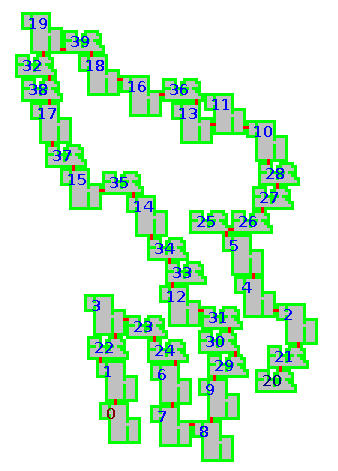
\includegraphics[scale=0.5]{img/mapsamples/mainpath}
\caption{Combinador parametrizado. Parámetros: camino principal (100), resto (0)
\label{fig:grfmainpath}}
\end{figure}


\begin{figure}[H]
\centering
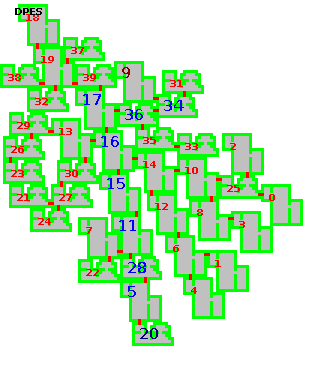
\includegraphics[scale=0.5]{img/mapsamples/altpathlength}
\caption{Combinador parametrizado. Parámetros: camino alternativo (100), resto (0)
\label{fig:grfaltpath}}
\end{figure}



\begin{figure}[H]
\centering
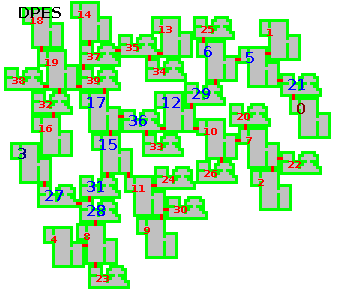
\includegraphics[scale=0.5]{img/mapsamples/branching}
\caption{Combinador parametrizado. Parámetros: branching (100), resto (0)
\label{fig:grfbranching}}
\end{figure}



\begin{figure}[H]
\centering
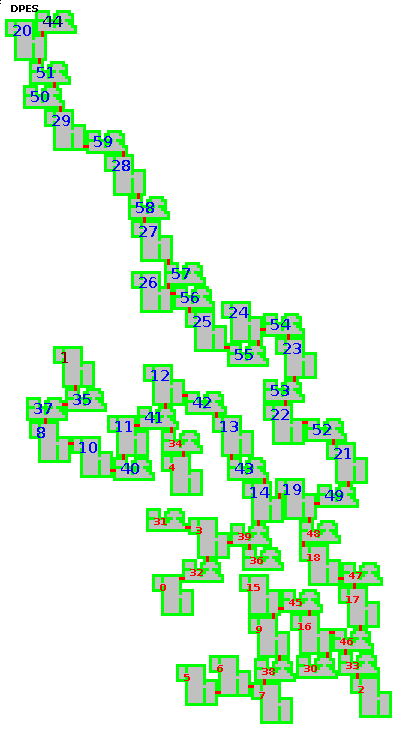
\includegraphics[scale=0.5]{img/mapsamples/MAINalt}
\caption{Combinador parametrizado. Parámetros: camino principal (5.8), camino alternativo (1), branching (0)
\label{fig:grfmainalt}}
\end{figure}


\begin{figure}[H]
\centering
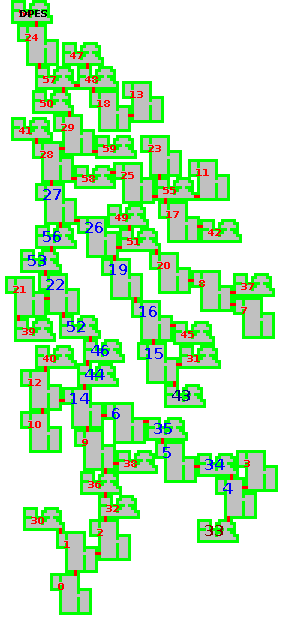
\includegraphics[scale=0.5]{img/mapsamples/MAINaltbranch}
\caption{Combinador parametrizado. Parámetros: camino principal (5.8), camino alternativo (1), branching (1)
\label{fig:grfmainaltbranch}}
\end{figure}



\begin{figure}[H]
\centering
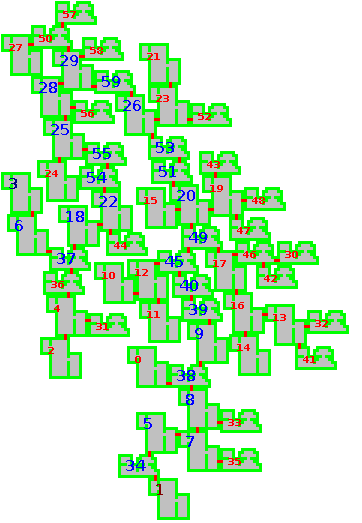
\includegraphics[scale=0.5]{img/mapsamples/adaptMAINaltbranch}
\caption{Combinador adaptativo. Attack/Decay (1/0.5). Parámetros: camino principal (10), camino alternativo (1), branching (1)
\label{fig:grfadaptMAINaltbranch}}
\end{figure}


\begin{figure}[H]
\centering
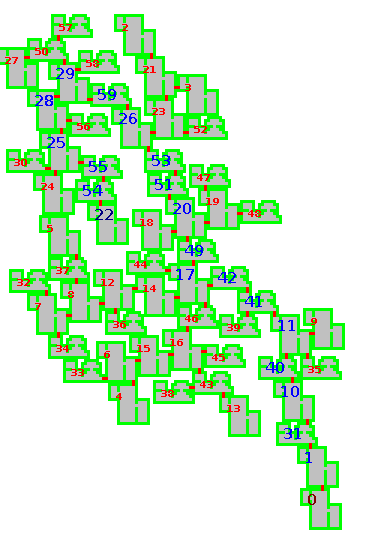
\includegraphics[scale=0.5]{img/mapsamples/adaptmainaltbranch}
\caption{Combinador adaptativo. Attack/Decay (1/0.5). Parámetros: camino principal (10), camino alternativo (10), branching (10)
\label{fig:grfadaptmainaltbranch}}
\end{figure}


\begin{figure}[H]
\centering
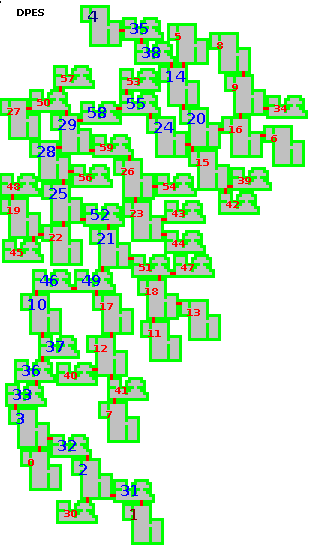
\includegraphics[scale=0.5]{img/mapsamples/adaptmainaltbranch2}
\caption{Combinador adaptativo. Attack/Decay (1.1/0.9). Parámetros: camino principal (10), camino alternativo (10), branching (10)
\label{fig:grfadaptmainaltbranch2}}
\end{figure}




\section{Eficiencia}

Recordemos que, aunque no se restringía un tamaño al escenario, se estima como tamaño máximo un escenario de 64x64 tiles. Aún así, para estresar el algoritmo, se han elaborado mapas con tamaños mayores. Por ejemplo, en uno de ellos el tamaño de habitación de 20x20, y en el mejor caso, con habitaciones de este tamaño cuadradas, podríamos tener 9 en un mapa de 64x64, pero veremos tiempos bastante buenos con una generación de este tipo hasta para escenarios de 30 habitaciones.

Como no se ha implementado en móvil, se ha considerado que un tiempo es bueno, cuando es menor de un segundo. Si es menor de dos segundos, también se considerará como aceptable. Aún así, habría que hacer una prueba real, que debido a que Java es la plataforma de elección para el desarrollo a Android, no sería complejo. En un caso real de un juego de móvil además, se presupone menor complejidad debido al sistema donde se ejecuta, y se puede entender que un tiempo aceptable de espera a la generación es hasta 10 segundos, y en esto se fundamenta la aceptación de menor de dos segundos como solución buena.

Destacar que las mediciones realizadas para comprobar el impacto de algunos parámetros se han usado sin tener en cuenta los demás. Al final, podremos ver una medición realizada sobre una configuración que se ha conseguido con tiempos muy buenos y calidad notable.

Las pruebas se han realizado en un portátil HP Compaq Presario V6000 con las siguientes características:

\begin{center}
	\begin{tabular}{ | c | c | }
\hline
Modelo procesador & AMD Athlon 64 X2 \\ 
Núcleos procesador & 2 (1 en uso) \\
Velocidad procesador & 1.7 Ghz \\
Caché procesador & 512 KB L2 \\
Memoria RAM & 1 GB \\
\hline
	\end{tabular}
\end{center}


\subsection{Impacto del factor divisor de movimientos}

Como se comentó anteriormente (ENLACE A ESTO), el factor de divisor de movimientos permite elegir un subconjunto de todos los movimientos posibles para cada paso de la generación.

Se han realizado pruebas con la configuración para el resto de parámetros como se indica en la tabla~\ref{table:cfgdpediv}, modificando el parámetro de divisor de movimientos para los valores 0.75, 0.85 y 0.95.

En la figura \ref{fig:grfdpedivs} se puede apreciar la influencia de este parámetro en los tiempos de generación. Normalmente, suelen dar mapas de buena calidad para los parámetros dados.

Ha de tenerse en cuenta que cuanto mayor son los posibles movimientos, menos influye el parámetro en la calidad de los mapas generados. Si aumentamos el tamaño de las habitaciones, podremos con seguridad aumentar el parámetro, ya que habrán muchos posibles movimientos asociados a cada habitación.

\begin{table}[H]
\begin{center}
	\begin{tabular}{ | c | c | }
\hline
 		Property & Value \\ \hline
DoorGenType & ALL \\ 
SolverType & BestSearch \\ 
CacheType & NO CACHE \\ 
\hline
	\end{tabular}
\end{center}
\caption{Configuración para divisor de movimientos}
\label{table:cfgdpediv}
\end{table}

\begin{table}[H]
\begin{center}
	\begin{tabular}{ | c | c | c | c | c | c | c | }
\hline
Tam. habs. & Modelos & Inst./modelo & Total habs. & 0.75f & 0.85f & 0.95f\\ \hline 
10 & 2 & 20 & 40 & 0.1763 & 0.1967 & 0.3667 \\ 
10 & 2 & 30 & 60 & 0.4945 & 0.6254 & 1.4392 \\ 
10 & 4 & 20 & 80 & 1.2336 & 1.6429 & 4.0735 \\ 
10 & 4 & 30 & 120 & 4.8805 & 6.6694 & 18.1853 \\ 
\hline
	\end{tabular}
\end{center}
\caption{Influencia del divisor de movimientos}
\label{table:dpediv}
\end{table}


\begin{figure}[H]
\centering
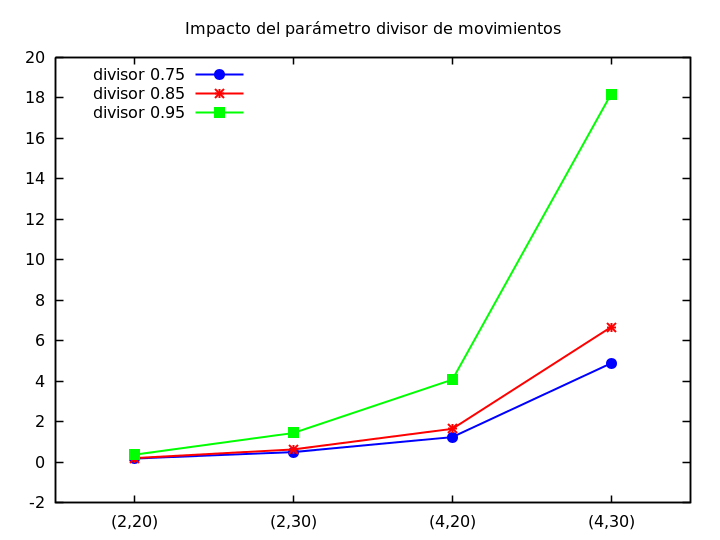
\includegraphics[scale=0.5]{img/dpedivs}
\caption{Gráfica de comparación de parámetro divisor de movimientos
\label{fig:grfdpedivs}}
\end{figure}



\subsection{Impacto de la generación de puertas aleatoria}

Gracias a este parámetro, podemos reducir el número de puertas potenciales de cada habitación. Así, se ha probado con un valor de 0.4, 0.6 y 0.8 para este aspecto. Cualquier valor es bueno, si tenemos en cuenta que el divisor de movimientos reducirá los posibles movimientos. Es decir, si elegimos una sola puerta potencial de todas las habitaciones y damos un valor muy alto del divisor de movimientos, obtendremos mapas de baja calidad, ya que estaremos limitando demasiado la exploración de posibilidades.

\begin{table}[H]
\begin{center}
	\begin{tabular}{ | c | c | }
\hline
 		Property & Value \\ \hline
DoorGenType & RANDOM \\ 
SolverType & BestSearch \\ 
BestSearch DPE Divisor & 1.0 \\ 
CacheType & NO CACHE \\ 
\hline
	\end{tabular}
\end{center}
\caption{Configuración del test de impacto de generación de puertas aleatorias}
\label{table:cfg-randoors}
\end{table}


\begin{table}[H]
\begin{center}
	\begin{tabular}{ | c | c | c | c | c | c | c | }
\hline
Tam. habs. & Modelos & Inst./modelo & Total & 0.8f & 0.6f & 0.4f \\ \hline 
10 & 4 & 8 & 32 & 4.6552 & 3.3017 & 1.7974 \\ 
10 & 4 & 10 & 40 & 9.8173 & 8.2366 & 4.1857 \\ 
10 & 6 & 8 & 48 & 29.2931 & 20.9267 & 15.4530 \\ 
10 & 6 & 10 & 60 & 69.2747 & 57.3447 & 34.6857 \\ 
\hline
	\end{tabular}
\end{center}
\caption{Test de impacto de generación de puertas aleatorias}
\label{table:randoors}
\end{table}


\begin{figure}[H]
\centering
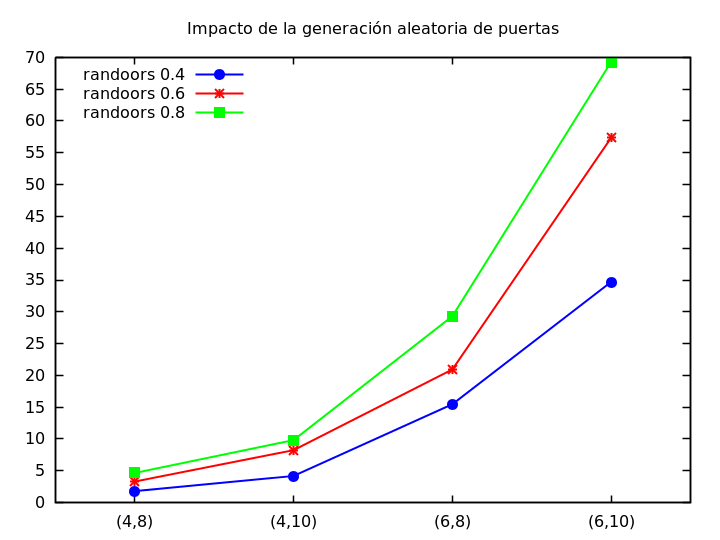
\includegraphics[scale=0.5]{img/randoors}
\caption{Gráfica de comparación de parámetro de generación de puertas aleatorias
\label{fig:grfrandoors}}
\end{figure}


\subsection{Impacto del Caché Refresher}

Este parámetro trabaja muy bien con la generación. En principio, si empleamos una caché que cachea siempre, obtenemos generaciones mediocres, sin llegar a ser excesivamente malas. Añadiendo este componente, podemos aumentar la calidad de los mapas de forma considerable y obteniendo tiempos bastante buenos.

En la figura \ref{fig:grfrefresher} se puede ver como se mejoran los tiempos empleando este parámetro.

\begin{table}[H]
\begin{center}
	\begin{tabular}{ | c | c | }
\hline
 		Property & Value \\ \hline
DoorGenType & ALL \\ 
SolverType & BestSearch \\ 
BestSearch DPE Divisor & 1.0 \\ 
CacheType & REFRESHER \\ 
\hline
	\end{tabular}
\end{center}
\caption{Configuración de test de impacto de caché refresher}
\label{table:cfg-refresher}
\end{table}



\begin{table}[H]
\begin{center}
	\begin{tabular}{ | c | c | c | c | c | c | c | c |}
\hline
Tam. habs. & Modelos & Inst./modelo & Total & N=2 & N=5 & N=10 \\ \hline 
6 & 4 & 10 & 40 & 1.3768 & 1.0284 & 0.7653 \\ 
6 & 4 & 15 & 60 & 6.7213 & 5.5230 & 3.4248 \\ 
6 & 6 & 10 & 60 & 8.7300 & 6.7349 & 5.5666 \\ 
6 & 6 & 15 & 90 & 43.7862 & 35.1948 & 26.3091 \\ 
\hline
	\end{tabular}
\end{center}
\caption{Test de impacto de caché refresher}
\label{table:refresher}
\end{table}


\begin{figure}[H]
\centering
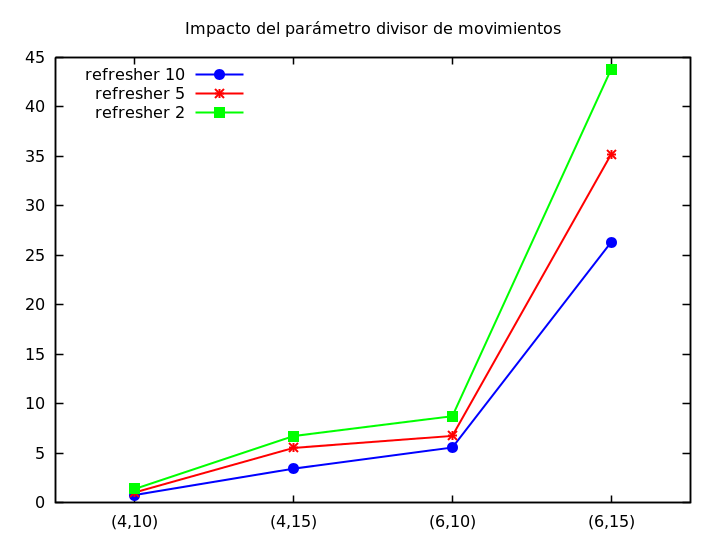
\includegraphics[scale=0.5]{img/refresher}
\caption{Gráfica de comparación de parámetro de caché refresher
\label{fig:grfrefresher}}
\end{figure}



\subsection{Ejemplo real optimizado}

Se ha elaborado una configuración optimizada para ejemplos que consideraremos reales de habitaciones desde 6x6 hasta 10x10, teniendo en cuenta que el tamaño del mapa puede rondar los 64x64 tiles. La configuración puede verse en la tabla \ref{table:cfg-optreal}.

En la figura \ref{grfoptreal} puede verse la evolución de los tiempos conforme aumentamos el número de modelos y de instancias por modelo para un tamaño de habitaciones de 6x6, y en la figura \ref{grfoptmid} para un tamaño de 10x10. Se observa como se obtienen tiempos muy buenos para ambos casos.

\begin{table}[H]
\begin{center}
	\begin{tabular}{ | c | c | }
\hline
 		Property & Value \\ \hline
DoorGenType & RANDOM \\ 
Refresher cache divisor & 10 \\ 
SolverType & BestSearch \\ 
BestSearch DPE Divisor & 0.9 \\ 
CacheType & REFRESHER \\ 
Random doors param & 0.5 \\ 
\hline
	\end{tabular}
\end{center}
\caption{Configuración para test real en dispositivos móviles}
\label{table:cfg-optreal}
\end{table}


\begin{table}[H]
\begin{center}
	\begin{tabular}{ | c | c | c | c | c | }
\hline
Tam. habs. & Modelos & Instancias/modelo & Total habs. & Tiempo \\ \hline 
6 & 5 & 1 & 5 & 0.0007 \\ 
6 & 5 & 2 & 10 & 0.0029 \\ 
6 & 5 & 3 & 15 & 0.0073 \\ 
6 & 5 & 4 & 20 & 0.0168 \\ 
6 & 10 & 1 & 10 & 0.0050 \\ 
6 & 10 & 2 & 20 & 0.0266 \\ 
6 & 10 & 3 & 30 & 0.0679 \\ 
6 & 10 & 4 & 40 & 0.1601 \\ 
6 & 15 & 1 & 15 & 0.0157 \\ 
6 & 15 & 2 & 30 & 0.0905 \\ 
6 & 15 & 3 & 45 & 0.3026 \\ 
6 & 15 & 4 & 60 & 0.6859 \\ 
6 & 20 & 1 & 20 & 0.0398 \\ 
6 & 20 & 2 & 40 & 0.2525 \\ 
6 & 20 & 3 & 60 & 0.7766 \\ 
6 & 20 & 4 & 80 & 2.0803 \\ 
\hline
	\end{tabular}
\end{center}
\caption{Test real en dispositivos móviles}
\label{table:optreal}
\end{table}

\begin{figure}[H]
\centering
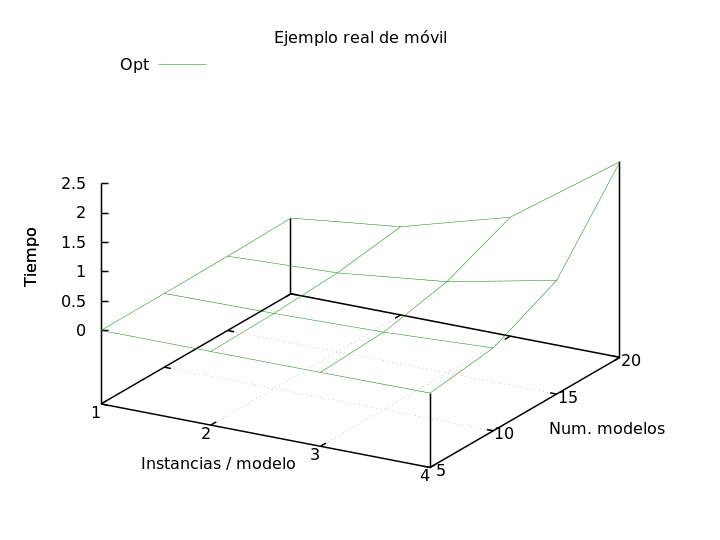
\includegraphics[scale=0.5]{img/opt-real}
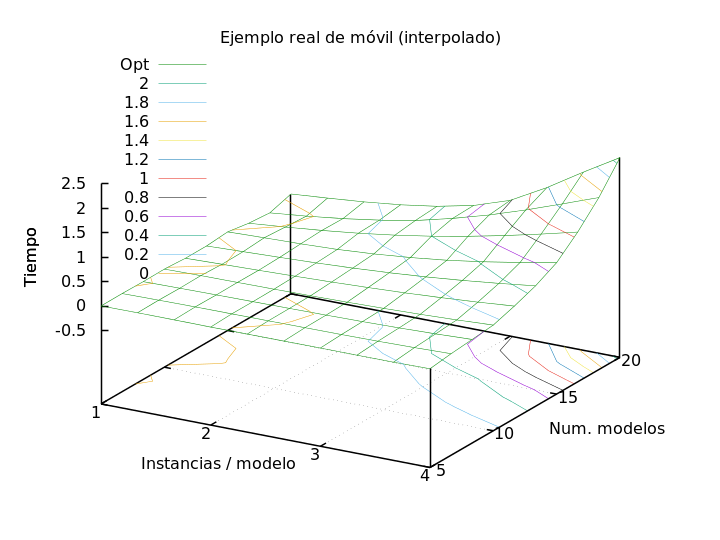
\includegraphics[scale=0.5]{img/opt-real-spl}
\caption{Gráfica de ejemplo óptimo real en móviles
\label{fig:grfoptreal}}
\end{figure}



\begin{table}[H]
\begin{center}
	\begin{tabular}{ | c | c | c | c | c | }
\hline
Tam. habs. & Modelos & Instancias/modelo & Total habs. & Tiempo \\ \hline 
10 & 5 & 1 & 5 & 0.0035 \\ 
10 & 5 & 2 & 10 & 0.0127 \\ 
10 & 5 & 3 & 15 & 0.0246 \\ 
10 & 10 & 1 & 10 & 0.0257 \\ 
10 & 10 & 2 & 20 & 0.1216 \\ 
10 & 10 & 3 & 30 & 0.1667 \\ 
10 & 15 & 1 & 15 & 0.1143 \\ 
10 & 15 & 2 & 30 & 0.3776 \\ 
10 & 15 & 3 & 45 & 0.8163 \\ 
\hline
	\end{tabular}
\end{center}
\caption{Test optimizado de tamaño medio}
\label{table:bsoptmedsamp}
\end{table}

\begin{figure}[H]
\centering
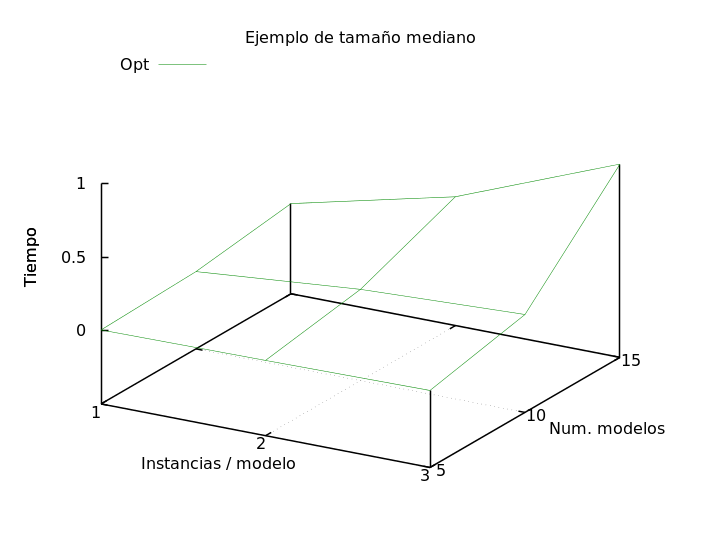
\includegraphics[scale=0.5]{img/opt-mid}
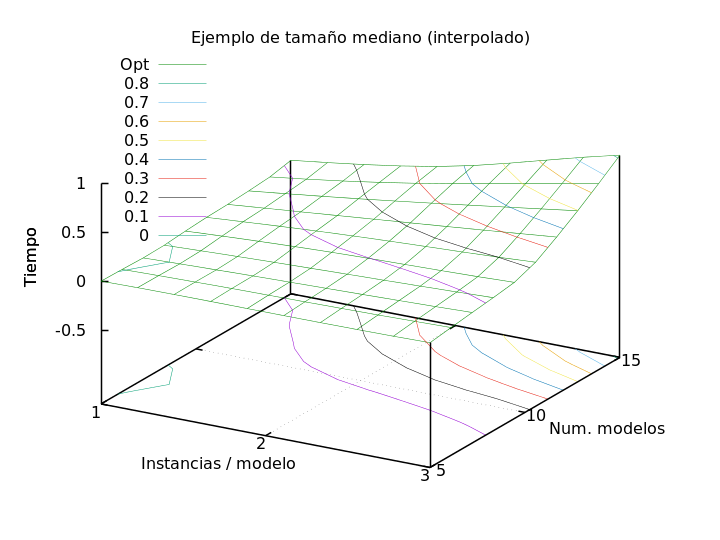
\includegraphics[scale=0.5]{img/opt-mid-spl}
\caption{Gráfica de ejemplo óptimo de tamaño medio
\label{fig:grfoptmid}}
\end{figure}









\subsection{Comparación ejemplo optimizado}

Si comparamos la configuración optimizada con ejemplos sin caché y cacheando siempre (pero no modificando el resto de parámetros), podemos ver como mejoramos bastante los tiempos. Además, obtenemos mapas con mejor calidad que si cacheáramos siempre.

\begin{table}[H]
\begin{center}
	\begin{tabular}{ | c | c | c | c | }
\hline
Property & NoCache & Always & Opt \\ \hline
DoorGenType & ALL & ALL & RANDOM \\
Random doors param & - & - & 0.5 \\
CacheType & - & ALWAYS & REFRESHER \\
Refresher cache divisor & - & - & 10 \\
SolverType & BestSearch & BestSearch & BestSearch \\
BestSearch DPE Divisor & 1.0 & 1.0 & 0.9 \\
\hline
	\end{tabular}
\end{center}
\caption{Configuración para test de comparación}
\label{table:cfg-comp}
\end{table}


\begin{table}[H]
\begin{center}
	\begin{tabular}{ | c | c | c | c | c | c | c | }
\hline
Tam. h. & Modelos & Inst./modelo & Total & NoCache & Always & Opt \\ \hline 
8 & 4 & 2 & 8 & 0.0333 & 0.0174 & 0.0030 \\ 
8 & 4 & 4 & 16 & 0.2818 & 0.0649 & 0.0123 \\ 
8 & 4 & 6 & 24 & 1.2533 & 0.1949 & 0.0354 \\ 
8 & 4 & 8 & 32 & 3.3727 & 0.4231 & 0.0780 \\ 
8 & 6 & 2 & 12 & 0.1696 & 0.0666 & 0.0107 \\ 
8 & 6 & 4 & 24 & 1.7436 & 0.2856 & 0.0481 \\ 
8 & 6 & 6 & 36 & 8.6428 & 1.0331 & 0.1302 \\ 
8 & 6 & 8 & 48 & 19.8587 & 2.7444 & 0.3155 \\ 
8 & 8 & 2 & 16 & 0.5825 & 0.2523 & 0.0210 \\ 
8 & 8 & 4 & 32 & 7.3917 & 1.1891 & 0.1030 \\ 
8 & 8 & 6 & 48 & 33.7262 & 3.6202 & 0.3438 \\ 
8 & 8 & 8 & 64 & 107.0144 & 9.6228 & 0.8999 \\ 
8 & 10 & 2 & 20 & 1.6964 & 1.0235 & 0.0643 \\
8 & 10 & 4 & 40 & 24.2987 & 3.1605 & 0.2243 \\
8 & 10 & 6 & 60 & 113.6830 & 11.2674 & 0.9700 \\
8 & 10 & 8 & 80 & 417.6313 & 28.2073 & 2.1928 \\
\hline
	\end{tabular}
\end{center}
\caption{Test de comparación}
\label{table:comp}
\end{table}


\begin{figure}[H]
\centering
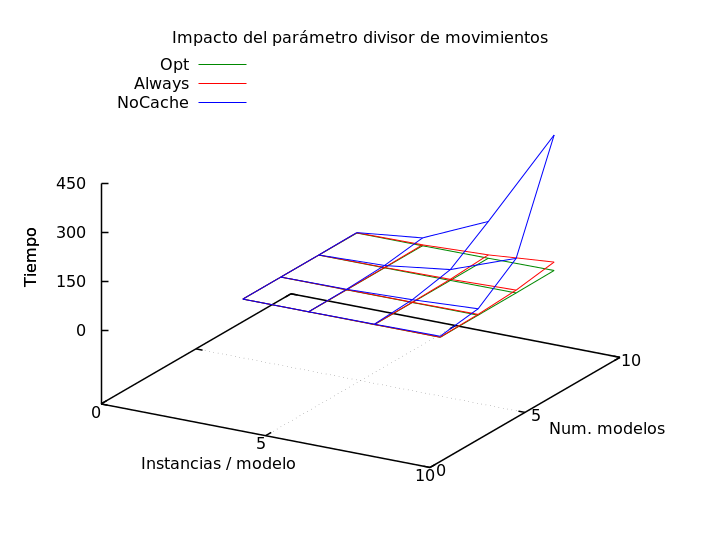
\includegraphics[scale=0.5]{img/comp-all}
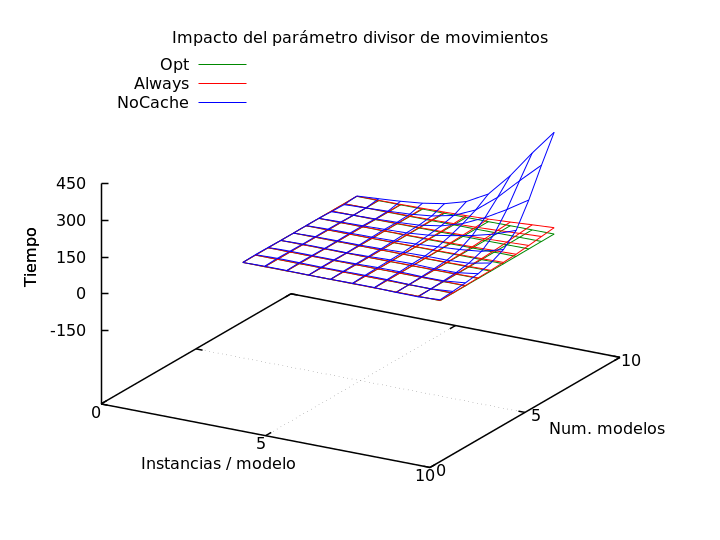
\includegraphics[scale=0.5]{img/comp-all-spl}
\caption{Gráfica de comparación entre AlwaysCache, NoCache y ejemplo optimizado
\label{fig:grfcompall}}
\end{figure}



\begin{figure}[H]
\centering
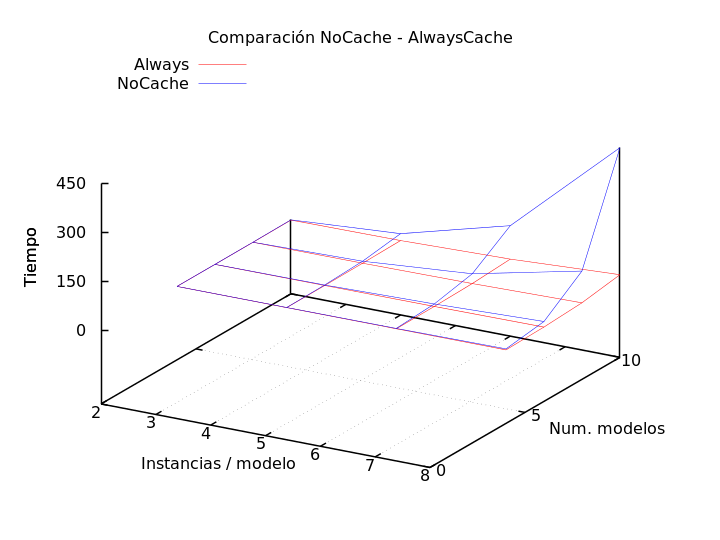
\includegraphics[scale=0.5]{img/comp-nc-alw}
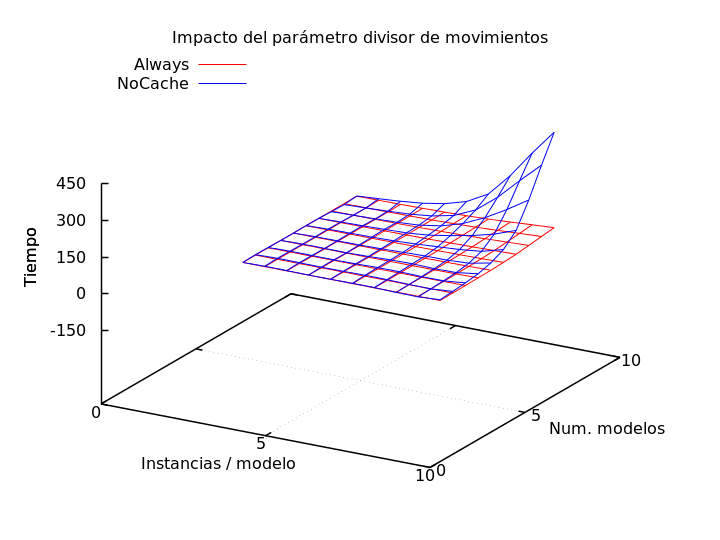
\includegraphics[scale=0.5]{img/comp-nc-alw-spl}
\caption{Gráfica de comparación entre AlwaysCache y NoCache
\label{fig:grfcompall}}
\end{figure}


\begin{figure}[H]
\centering
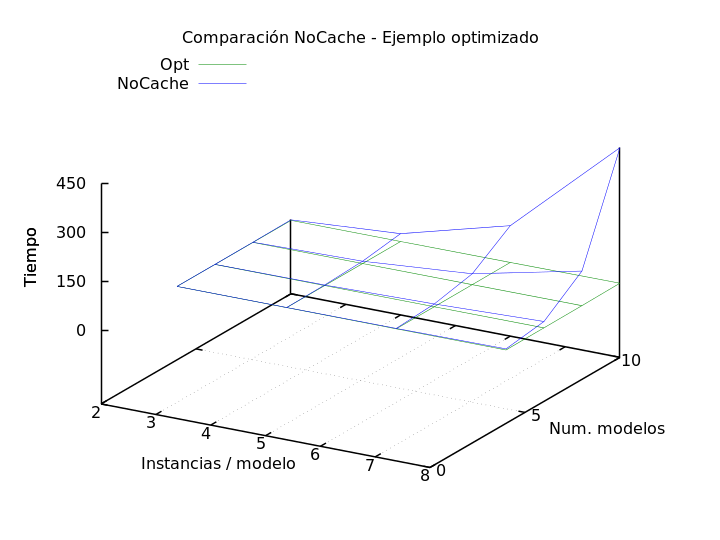
\includegraphics[scale=0.5]{img/comp-nc-opt}
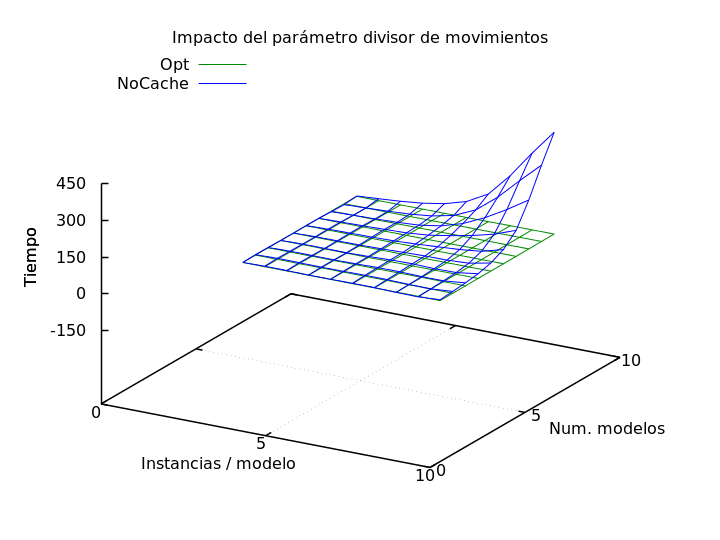
\includegraphics[scale=0.5]{img/comp-nc-opt-spl}
\caption{Gráfica de comparación entre NoCache y ejemplo optimizado
\label{fig:grfcompall}}
\end{figure}






\begin{figure}[H]
\centering
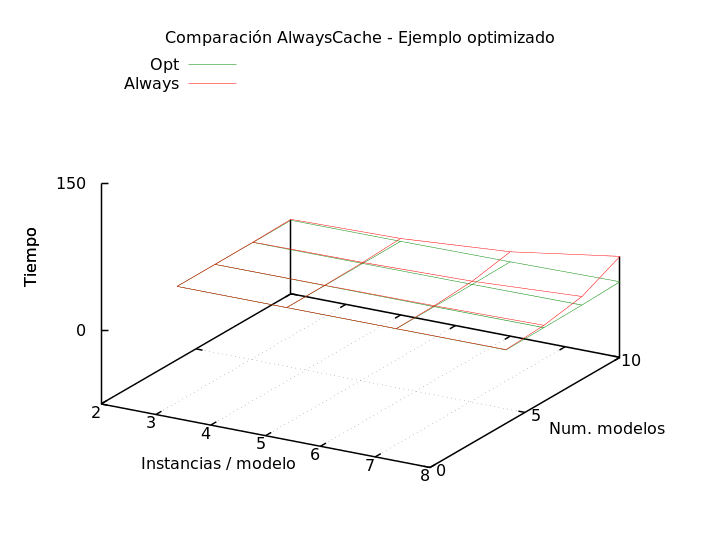
\includegraphics[scale=0.5]{img/comp-alw-opt}
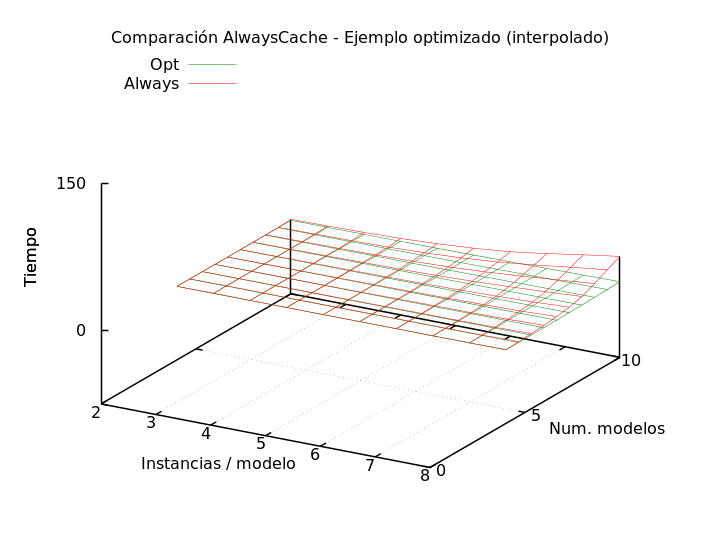
\includegraphics[scale=0.5]{img/comp-alw-opt-spl}
\caption{Gráfica de comparación entre AlwaysCache y ejemplo optimizado
\label{fig:grfcompall}}
\end{figure}








\subsection{Muchos tipos de habitación}

Por último, hemos querido hacer un ejemplo donde la diversidad de modelos es muy alta. Es decir, se empleará un número alto de modelos y bajo de instancias por modelo.

En la gráfica \ref{fig:optvar}, podemos ver un caso que tarda un tiempo excesivo de 7 segundos. Para ello, se ha realizado una modificación en la configuración, obteniendo un arreglo del mismo que puede observarse en la figura \ref{fig:varfixcmp}.

\begin{table}[H]
\begin{center}
	\begin{tabular}{ | c | c | }
\hline
 		Property & Value \\ \hline
DoorGenType & RANDOM \\ 
Refresher cache divisor & 10 \\ 
SolverType & BestSearch \\ 
BestSearch DPE Divisor & 0.9 \\ 
CacheType & REFRESHER \\ 
Random doors param & 0.5 \\ 
\hline
	\end{tabular}
\end{center}
\caption{Configuración test con variabilidad en habitaciones}
\label{table:cfg-optvarsample}
\end{table}


\begin{table}[H]
\begin{center}
	\begin{tabular}{ | c | c | c | c | c | }
\hline
Tam. habs. & Modelos & Instancias/modelo & Total habs. & Tiempo \\ \hline 
6 & 20 & 1 & 20 & 0.0395 \\ 
6 & 20 & 2 & 40 & 0.2505 \\ 
6 & 30 & 1 & 30 & 0.1479 \\ 
6 & 30 & 2 & 60 & 0.9846 \\ 
6 & 40 & 1 & 40 & 0.4307 \\ 
6 & 40 & 2 & 80 & 2.9426 \\ 
6 & 50 & 1 & 50 & 0.9980 \\ 
6 & 50 & 2 & 100 & 7.6388 \\ 
\hline
	\end{tabular}
\end{center}
\caption{Test con variabilidad en habitaciones}
\label{table:optvarsample}
\end{table}


\begin{figure}[H]
\centering
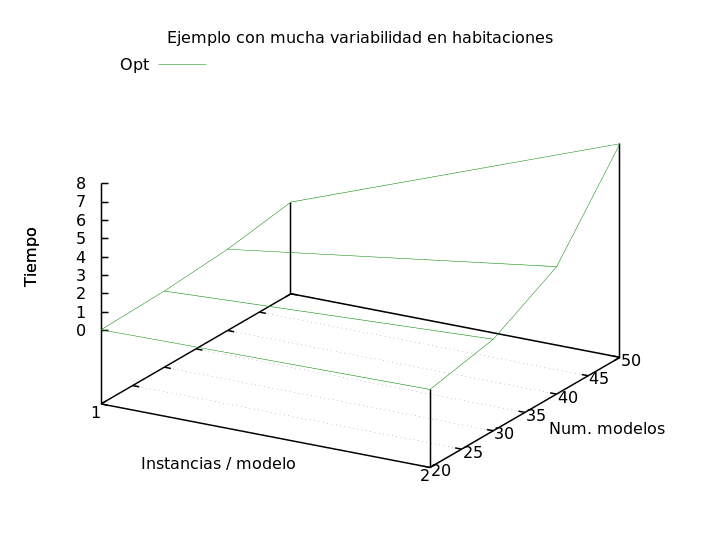
\includegraphics[scale=0.5]{img/opt-var}
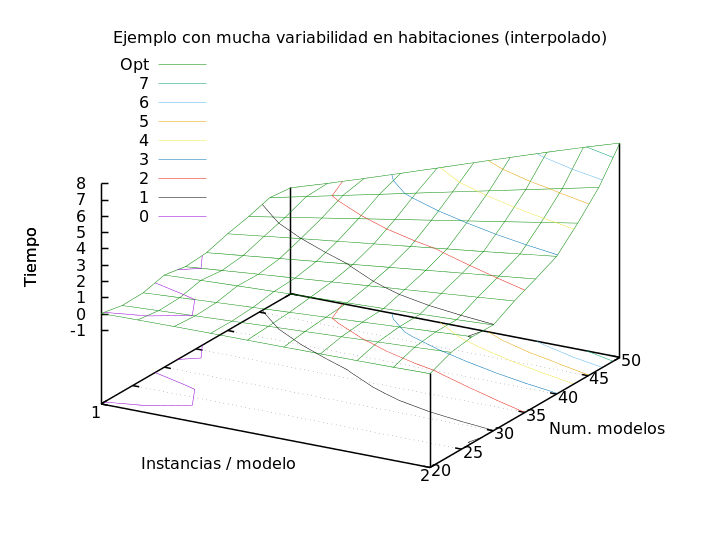
\includegraphics[scale=0.5]{img/opt-var-spl}
\caption{Gráfica de ejemplo variable con muchos modelos de habitaciones
\label{fig:grfoptvar}}
\end{figure}





\begin{table}[H]
\begin{center}
	\begin{tabular}{ | c | c | }
\hline
 		Property & Value \\ \hline
DoorGenType & RANDOM \\ 
SolverType & BestSearch \\ 
BestSearch DPE Divisor & 0.5 \\ 
CacheType & ALWAYS \\ 
Random doors param & 0.3 \\ 
\hline
	\end{tabular}
\end{center}
\caption{Configuración para el arreglo del último caso en test con variabilidad en habitaciones}
\label{table:cfg-optvarfix}
\end{table}


\begin{table}[H]
\begin{center}
	\begin{tabular}{ | c | c | c | c | c | }
\hline
Tam. habs. & Modelos & Instancias/modelo & Total habs. & Tiempo \\ \hline 
6 & 20 & 1 & 20 & 0.1615 \\ 
6 & 20 & 2 & 40 & 0.1523 \\ 
6 & 30 & 1 & 30 & 0.0494 \\ 
6 & 30 & 2 & 60 & 0.2139 \\ 
6 & 40 & 1 & 40 & 0.1108 \\ 
6 & 40 & 2 & 80 & 0.6791 \\ 
6 & 50 & 1 & 50 & 0.2222 \\ 
6 & 50 & 2 & 100 & 1.3180 \\ 

\hline
	\end{tabular}
\end{center}
\caption{Arreglo del último caso en test con variabilidad en habitaciones}
\label{table:optvarfix}
\end{table}



\begin{figure}[H]
\centering
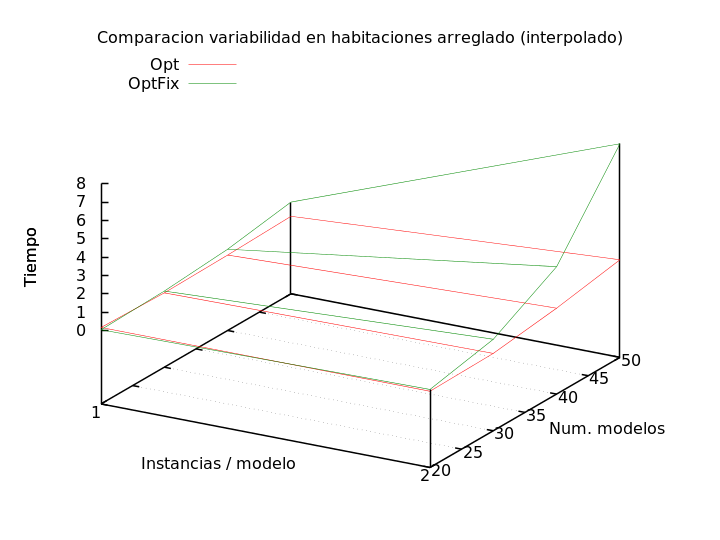
\includegraphics[scale=0.5]{img/opt-varfix}
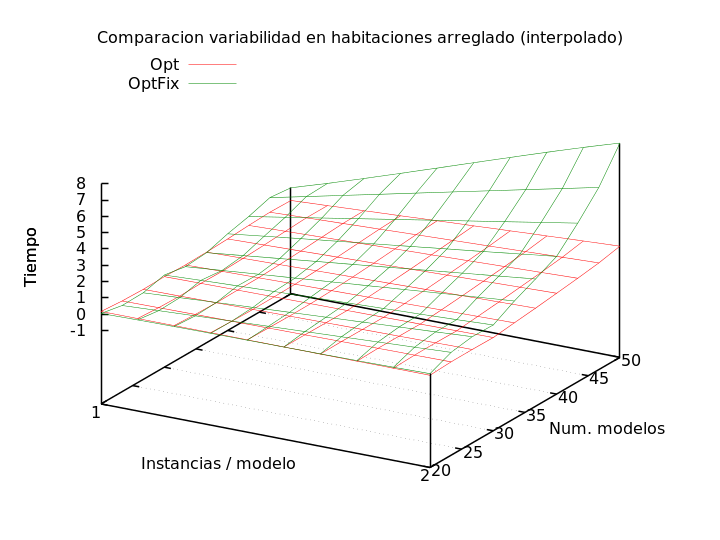
\includegraphics[scale=0.5]{img/opt-varfix-cmp-spl}
\caption{Gráfica de comparación entre ejemplo variable y arreglado
\label{fig:grfvarfixcmp}}
\end{figure}



\begin{figure}[H]
\centering
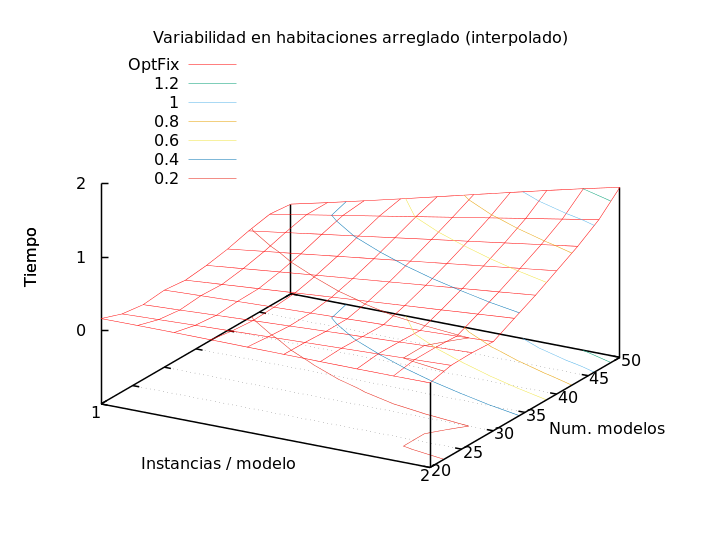
\includegraphics[scale=0.5]{img/opt-varfix-spl}
\caption{Arreglo de ejemplo variable
\label{fig:grfvarfix}}
\end{figure}
   % 
\chapter{Trabajo futuro.}\label{cap:capitulo8}


\section{Soporte para capas.}

Es arte, no interfiere en el sistema, pero viene bien. Dependiente del soporte.


\section{Mapa de tamaño autoajustable}


\section{Otros fitness}


\section{Portar a móvil}

Debido a los tiempos de ejecución y a la fitness caché, seguro que se puede.

\section{Otros fitness caché}


\section{Backtracking con guardado de movimientos}

Guardar no mejores, pero si muy buenos.
   % 
\begin{thebibliography}{99}

\addcontentsline{toc}{chapter}{Bibliografía.}

\bibitem{lucasarts} \href{https://es.wikipedia.org/wiki/LucasArts}{LucasArts Wikipedia page}

\bibitem{lod} \href{http://www.techopedia.com/definition/11791/level-of-detail-lod}{Techopedia LOD page}

\bibitem{voxel} Voxel wikipedia

\bibitem{quadtree} Quadtree wikipedia

\bibitem{octree} Octree wikipedia

\bibitem{brush} Brush wikipedia

\bibitem{quake} Quake wikipedia

\bibitem{rlike} RogueLike wikipedia

\bibitem{costgames} \href{https://en.wikipedia.org/wiki/List_of_most_expensive_video_games_to_develop}{List of most expensive video games to develop.}

\bibitem{gdroles1} \href{http://creativeskillset.org/creative_industries/games/job_roles}{Gamedev Job Roles at CreativeSkillSet}

\bibitem{gdroles2} \href{https://en.wikipedia.org/wiki/Video_game_development#Roles}{Video Game Development Wikipedia page}

\bibitem{dmscn} DemoScene wikipedia

\bibitem{texmodproc} http://www.amazon.com/Texturing-Modeling-Third-Edition-Procedural/dp/1558608486

\bibitem{libnoise} http://libnoise.sourceforge.net/tutorials/tutorial3.html

\bibitem{amitvoronoi} http://www-cs-students.stanford.edu/~amitp/game-programming/polygon-map-generation/

\bibitem{labygen} http://weblog.jamisbuck.org/2011/2/7/maze-generation-algorithm-recap

\bibitem{tinykeep} \href{http://www.reddit.com/r/gamedev/comments/1dlwc4/procedural_dungeon_generation_algorithm_explained/}{Explicación del algoritmo de generación de mazmorras empleado en TinyKeep.}

\end{thebibliography}









%%  Apendices
%%%%%%%%%%%%%%%%%%%%%%%%%%%%%%%%%%%%%%%%%%%%%%%%%%%%%%%%%%%%%%%%%%%%%%

%\appendix
%\include{apendice}  % Puedo poner la ontología OSMV y la arquitectura de OW

%%  Bibliografia
%%%%%%%%%%%%%%%%%%%%%%%%%%%%%%%%%%%%%%%%%%%%%%%%%%%%%%%%%%%%%%%%%%%%%%
\newpage
\addcontentsline{toc}{chapter}{Bibliografía}
\bibliographystyle{alpha}
\bibliography{biblio/bibliografia.tex}

\end{document}

